% !TeX spellcheck = pl_PL-Polish
%\documentclass[xcolor=pdftex,dvipsnames,table]{beamer}
%\documentclass[dvipsnames]{beamer}
\documentclass[11pt, xcolor={dvipsnames,svgnames},aspectratio=169]{beamer}
%\hypersetup{colorlinks}1
\usepackage{etex} % tikz needs it
\usepackage[utf8]{inputenc}
\usepackage{polski}
\usepackage[OT4]{fontenc} % doesn't change - default, and best?
%\usepackage[T1]{fontenc} % thinner, a bit more machine like
%\usepackage{times} % serif
\usepackage{amsfonts}
\usepackage{amsmath}
\usepackage{amsthm}
\usepackage{amsbsy}
\usepackage{amscd}
\usepackage{bbm}
\usepackage[mathscr]{eucal} 
%\usepackage{subfigure}
\usepackage{pifont}
\usepackage{color}
\usepackage{booktabs}
\usepackage{colortbl}
\usepackage{marvosym}
\usepackage{wasysym}
\usepackage[normalem]{ulem}
\usepackage{multicol}
\usepackage[makeroom]{cancel}
\usepackage{soul}
\definecolor{orange}{rgb}{0.75,0.33,0}
\newcommand{\myemph}[1]{\textcolor{orange}{#1}}

%\usepackage{tikz}
%\usetikzlibrary{arrows,shapes,snakes,automata,backgrounds,petri}

%\usepackage{beamerthemeshadow}
%\usecolortheme{crane}
%\usecolortheme{seahorse}
%\usetheme{default} 
%\usetheme[secheader]{Boadilla} 
%\usetheme{Luebeck} 
%\usecolortheme{seahorse}
%\usecolortheme{dolphin}

%\usetheme{default}
%\usetheme[backgroundimagefile=title.png,useblacktitletext,opacity=0]{diepen}
%\usefonttheme{structurebold}

%\definecolor{iipred}{RGB}{99,36,35}
%\usecolortheme[RGB={99,36,35}]{structure}
%\setbeamertemplate{navigation symbols}{}
%\setbeamertemplate{navigation symbols}{\insertframenumber/\inserttotalframenumber}

%\newcommand{\iitisSmall}{\includegraphics[width=0.06\textwidth]{iitisSmallest.png}}

\usepackage{isomath}
\usepackage{soul}
%\usepackage{ctable}

\renewcommand\mathfamilydefault{\rmdefault}

\newcommand{\attr}[1]{\tiny\begin{flushright}(source: #1)\end{flushright}\normalsize
}
\newcommand{\attrl}[1]{\tiny\begin{flushleft}(source: #1)\end{flushleft}\normalsize
}


%\newcommand{\source}[1]{\tiny\begin{flushright}(źródło ilustacji: \texttt{#1})\end{flushright}\normalsize}

 
\usetheme{iitisask}
\title[]{Statystyczne metody uczenia maszynowego -- wprowadzenie}
\author{Przemysław Głomb}
\date{redaktor pomocniczy: Bartłomiej Gardas}

\theoremstyle{plain}
\newcommand{\scaly}{0.7}

 	
 	
 \theoremstyle{plain}
 	
% 	\section{Sekcja 1}
% 	\subsection{Podsekcja 1}
% 	\subsubsection{Podpodsekcja 1}
% 	
% 	\begin{frame}{Tytuł slajdu}
% 		\framesubtitle{Podtytuł slajdu}
% 		\begin{itemize}
% 			\item \lipsum[1]
% 		\end{itemize}
% 	\end{frame}
% 	
% 	\begin{frame}{Tytuł slajdu}
% 		\begin{block}{Tytuł bloku}
% 			\lipsum[1]
% 		\end{block}
% 	\end{frame}
% 	
% 	\begin{frame}{Tytuł slajdu}
% 		\begin{theorem}
% 			$\ket{x}=[0,1]^\dagger$
% 		\end{theorem}
% 	\end{frame}
% 	
% 	\begin{frame}{Tytuł slajdu}
% 		\begin{exampleblock}{Przykład 1}
% 			$\ket{x}=[0,1]^\dagger$
% 		\end{exampleblock}
% 	\end{frame}
 	
 
 
\begin{document}


\frame{\maketitle}


% \AtBeginSection[]
% {
%    \begin{frame}
%        \frametitle{Plan wykładu}
%        \tableofcontents[currentsection]
%    \end{frame}
% }


\newcommand{\plotsize}{0.3}
\newcommand{\plotsizeone}{0.6}
\newcommand{\plotsizesm}{0.15}


\section{Analiza przykładowego sygnału}


\begin{frame}
	\frametitle{Dane -- przykładowy sygnał}
	\begin{center}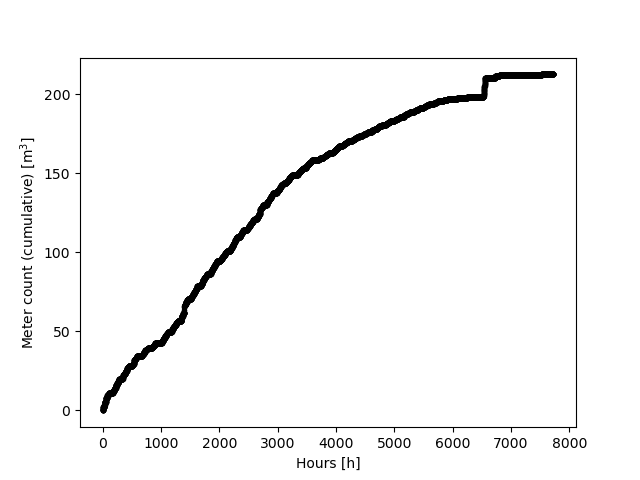
\includegraphics[width=\plotsizeone\textwidth]{images/sig1.png}\end{center}
\end{frame}
\begin{frame}
	\frametitle{Dane -- przykładowy sygnał (zoom)}
	\begin{center}
		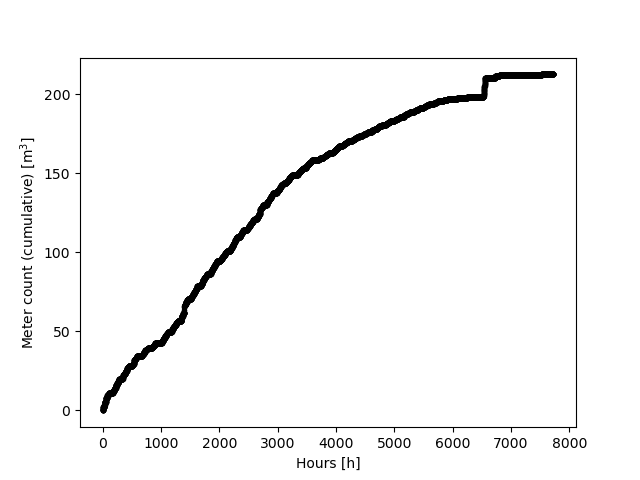
\includegraphics[width=\plotsize\textwidth]{images/sig1.png}
		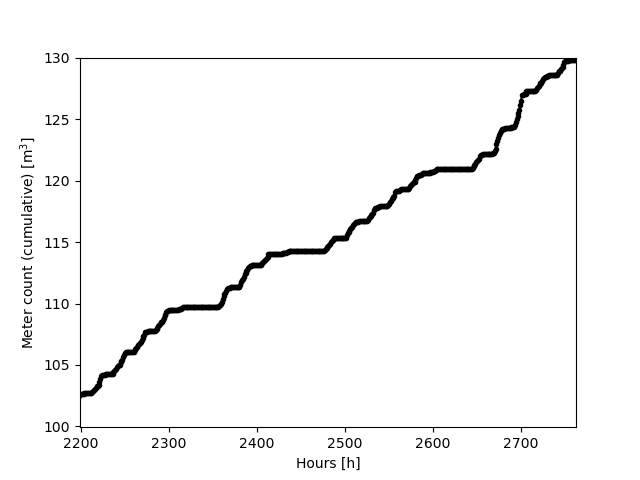
\includegraphics[width=\plotsize\textwidth]{images/sig1a.png}\\
		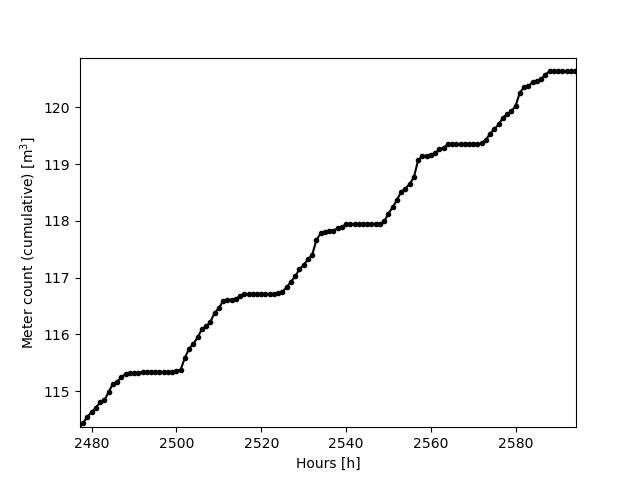
\includegraphics[width=\plotsize\textwidth]{images/sig1aa.png}
		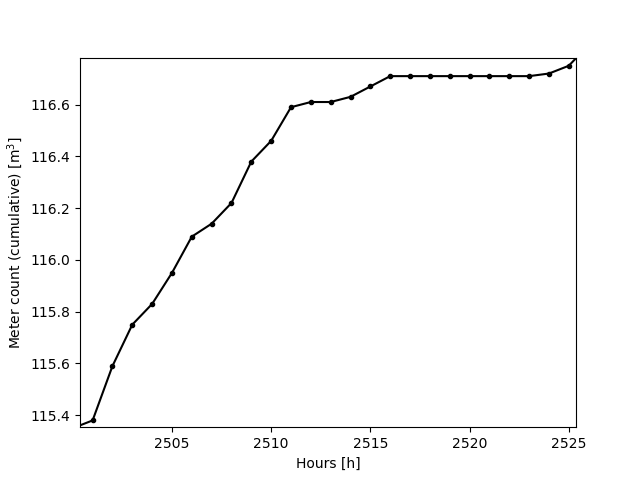
\includegraphics[width=\plotsize\textwidth]{images/sig1aaa.png}
	\end{center}
\end{frame}
\begin{frame}
	\frametitle{Dane -- przykładowy sygnał -- obserwacje/cechy}
	\begin{enumerate}
		\item Szereg czasowy
		\item<2-> Kumulatywne zliczanie impulsów -- sygnał kumulatywny (ang. integrative) -- różnicowanie (ang. differentiation)
			\begin{description}
				\item[$\rightarrow$] Sygnał, sygnał po różnicowaniu, sygnał po scałkowaniu
			\end{description}
	\end{enumerate}
\end{frame}
\begin{frame}
	\frametitle{Dane -- przykładowy sygnał -- różnicowanie}
	\begin{center}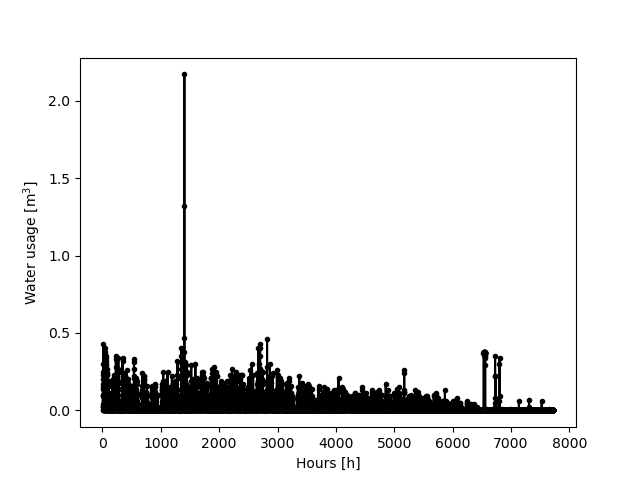
\includegraphics[width=\plotsizeone\textwidth]{images/sig1d.png}\end{center}
\end{frame}
\begin{frame}
	\frametitle{Dane -- przykładowy sygnał -- różnicowanie}
	\begin{center}
		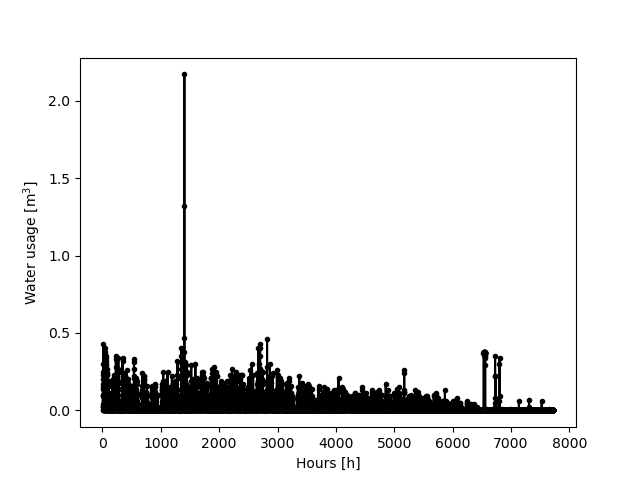
\includegraphics[width=\plotsize\textwidth]{images/sig1d.png}
		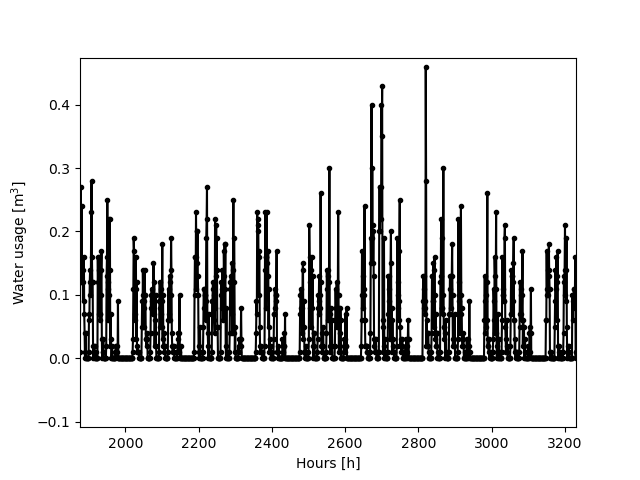
\includegraphics[width=\plotsize\textwidth]{images/sig1dd.png}\\
		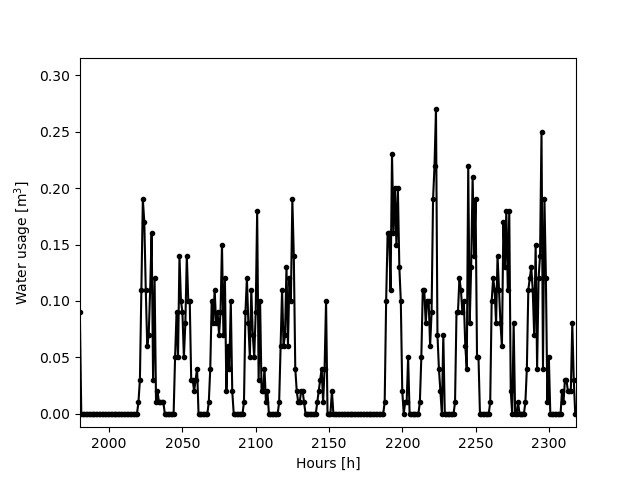
\includegraphics[width=\plotsize\textwidth]{images/sig1ddd.png}
		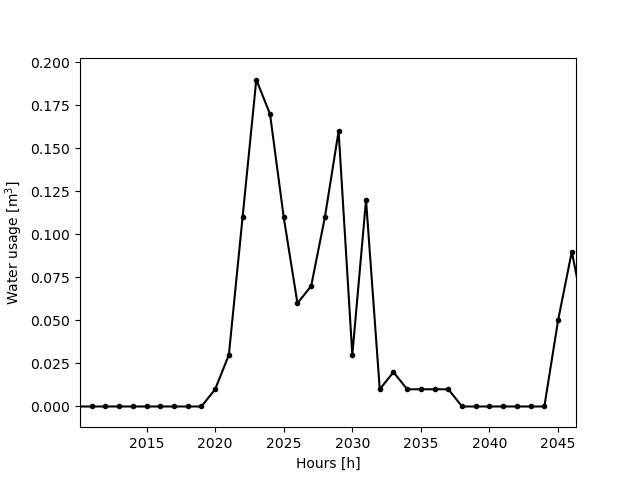
\includegraphics[width=\plotsize\textwidth]{images/sig1dddd.png}
	\end{center}
\end{frame}
\begin{frame}
	\frametitle{Dane -- przykładowy sygnał -- obserwacje/cechy}
	\begin{enumerate}
	\item Szereg czasowy
	\item Kumulatywne zliczanie impulsów -- sygnał kumulatywny (ang. integrative) -- różnicowanie (ang. differentiation)
		\begin{description}
			\item[$\rightarrow$] Sygnał, sygnał po różnicowaniu, sygnał po scałkowaniu
		\end{description}
	\item Cykl -- dobowy, tygodniowy
		\begin{description}
			\item[$\rightarrow$] Cykle, sezonowość
		\end{description}
	\item<2-> Trend -- zmienny
	\item<3-> Pojedyncze zdarzenia -- anomalie
	\item<4-> Wartości liczbowe (min/max, typowe, rozkład wartości)
	\end{enumerate}
	\begin{center}
		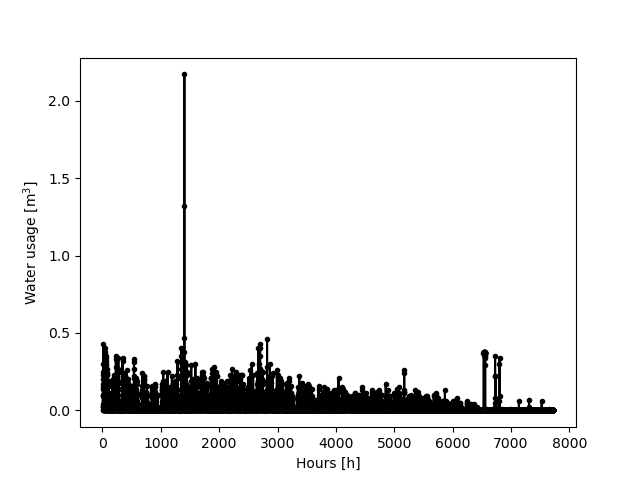
\includegraphics[width=\plotsizesm\textwidth]{images/sig1d.png}
		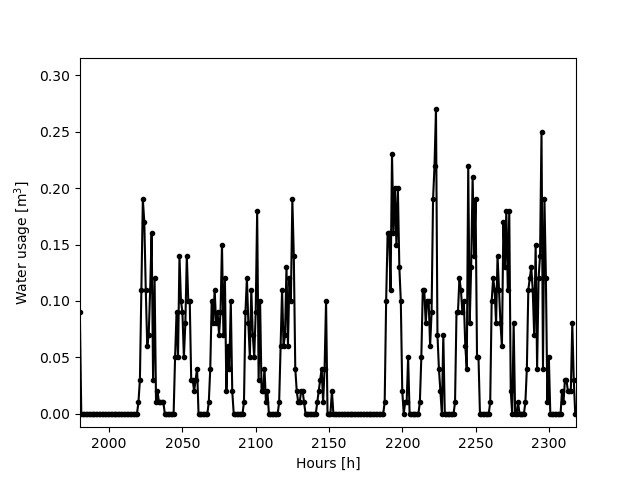
\includegraphics[width=\plotsizesm\textwidth]{images/sig1ddd.png}
	\end{center}
\end{frame}
\begin{frame}
	\frametitle{Bazy danych, weryfikacja danych}
	\begin{enumerate}
		\item Dane, informacja, wiedza
		\item<2-> Reprezentacja danych -- sposób zapisu w pamięci komputera
		\item<3-> Baza danych -- zorganizowany zbiór danych
		\item<4-> Weryfikacja
			\begin{enumerate}
				\item Poprawność i spójność
				\item Weryfikacja merytoryczna -- ,,sens'' danych, znaczenie, kontekst, \dots
					\begin{enumerate}
						\item Anomalie -- odstępstwa od ,,normy''
						\item Wystąpienie znanych problemów -- detekcja/klasyfikacja
					\end{enumerate}
			\end{enumerate}
	\end{enumerate}
	\only<5>{
	\begin{center}
		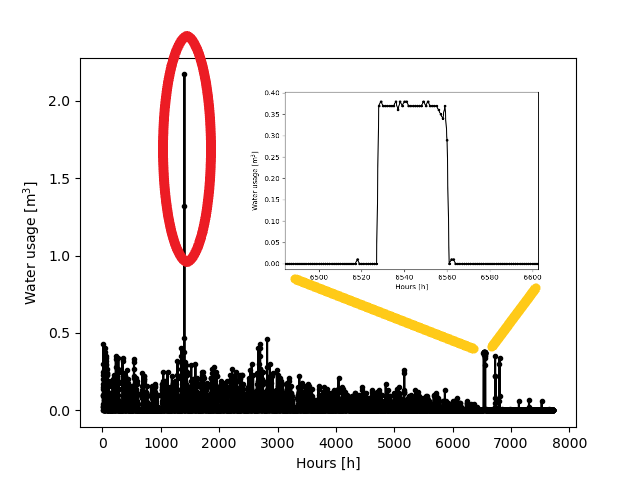
\includegraphics[width=0.3\textwidth]{images/ano.png}
	\end{center}}
\end{frame}


\section{Weryfikacja statystyczna -- MAD}


\begin{frame}
	\frametitle{Statystyki opisowe -- opis sygnału}
	\begin{enumerate}
		\item \sout{Szereg czasowy} $\rightarrow$ histogram
	\end{enumerate}
	\begin{center}
		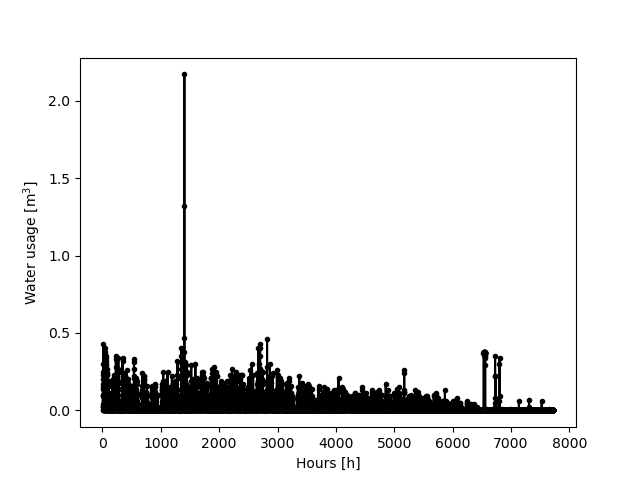
\includegraphics[width=\plotsize\textwidth]{images/sig1d.png} $\rightarrow$
		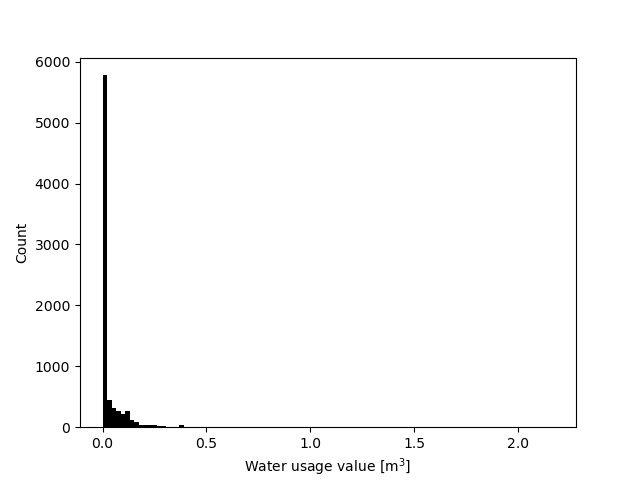
\includegraphics[width=\plotsize\textwidth]{images/hist.png}
	\end{center}
\end{frame}
\begin{frame}
	\frametitle{Statystyki opisowe -- opis sygnału -- histogram}
	\begin{center}
		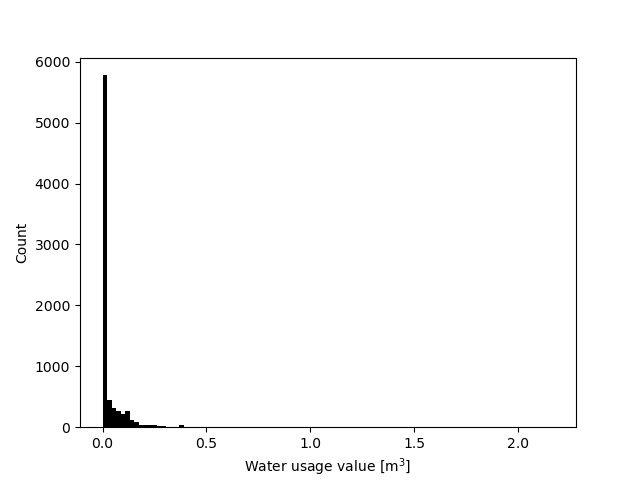
\includegraphics[width=0.49\textwidth]{images/hist.png}
		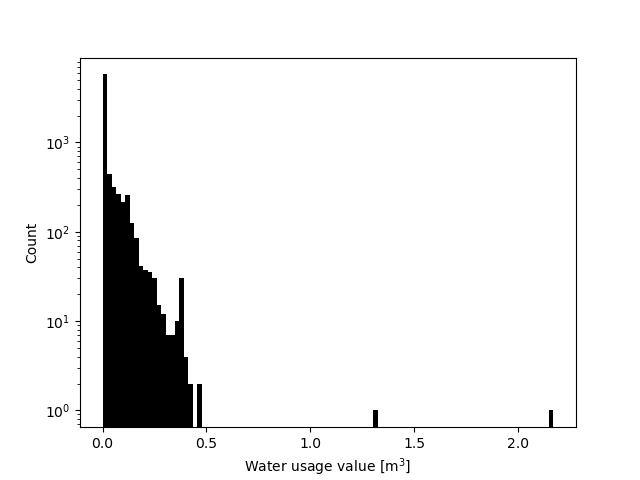
\includegraphics[width=0.49\textwidth]{images/histlog.png}
	\end{center}
\end{frame}
\begin{frame}
	\frametitle{Statystyki opisowe -- opis sygnału}
	\begin{description}
		\item[średnia] $\mu=0.028\qquad \mu=\frac{1}{n}\sum_i^n x_i$
	\end{description}
	\begin{center}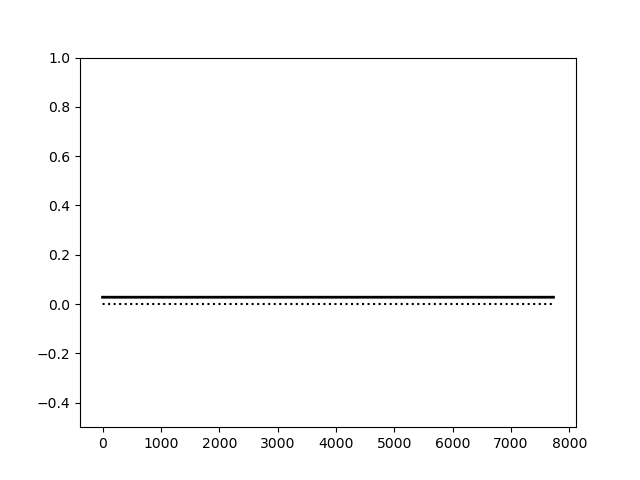
\includegraphics[width=0.45\textwidth]{images/m.png}\end{center}
\end{frame}
\begin{frame}
	\frametitle{Statystyki opisowe -- opis sygnału}
	\begin{description}
		\item[średnia] $\mu=0.028\qquad \mu=\frac{1}{n}\sum_i^n x_i$
		\item[wariancja] $\sigma^2=0.004 \qquad \sigma^2=\frac{1}{n}\sum_i^n (\mu - x_i)^2 \qquad \sigma=0.064$
	\end{description}
	\begin{center}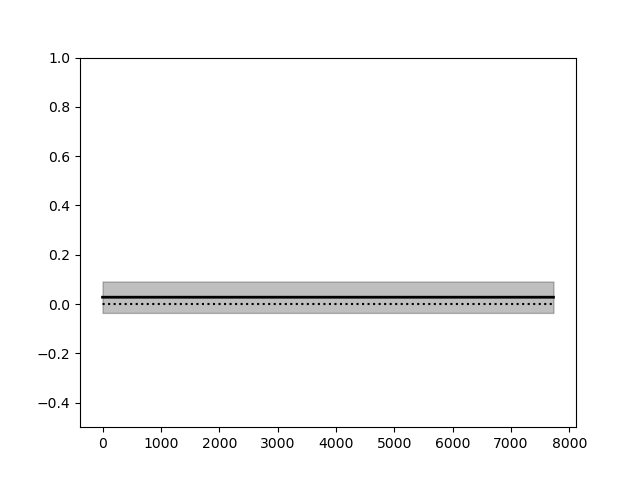
\includegraphics[width=0.45\textwidth]{images/mv.png}\end{center}
\end{frame}
\begin{frame}
	\frametitle{Statystyki opisowe -- opis sygnału}
	\begin{description}
		\item[średnia] $\mu=0.028\qquad \mu=\frac{1}{n}\sum_i^n x_i$
		\item[wariancja] $\sigma^2=0.004 \qquad \sigma^2=\frac{1}{n}\sum_i^n (\mu - x_i)^2 \qquad \sigma=0.064$
		\item[skośność] $s=8.234$
	\end{description}
	\begin{center}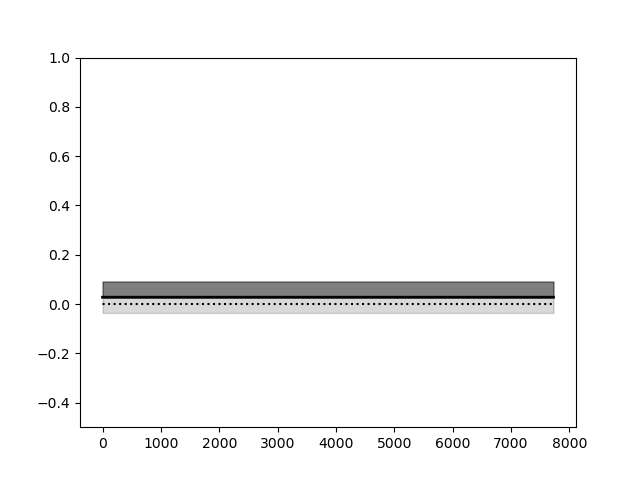
\includegraphics[width=0.45\textwidth]{images/mvs.png}\end{center}
\end{frame}
\begin{frame}
	\frametitle{Statystyki opisowe -- opis sygnału}
	\begin{description}
		\item[średnia] $\mu=0.028\qquad \mu=\frac{1}{n}\sum_i^n x_i$
		\item[wariancja] $\sigma^2=0.004 \qquad \sigma^2=\frac{1}{n}\sum_i^n (\mu - x_i)^2 \qquad \sigma=0.064$
		\item[skośność] $s=8.234$
		\item[kurtoza] $k=193.664$ 
	\end{description}
	\begin{center}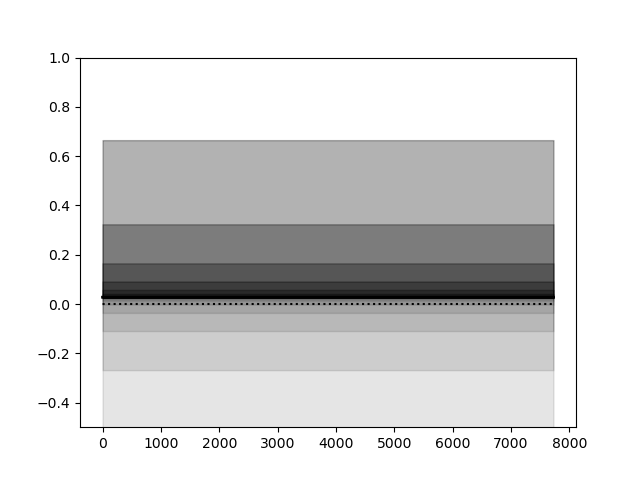
\includegraphics[width=0.45\textwidth]{images/mvsk.png} \end{center}
\end{frame}
\begin{frame}
	\frametitle{Statystyki opisowe -- opis sygnału}
	\begin{description}
		\item[średnia] $\mu=0.028\qquad \mu=\frac{1}{n}\sum_i^n x_i$
		\item[wariancja] $\sigma^2=0.004 \qquad \sigma^2=\frac{1}{n}\sum_i^n (\mu - x_i)^2 \qquad \sigma=0.064$
		\item[skośność] $s=8.234$
		\item[kurtoza] $k=193.664$ 
	\end{description}
	\begin{center}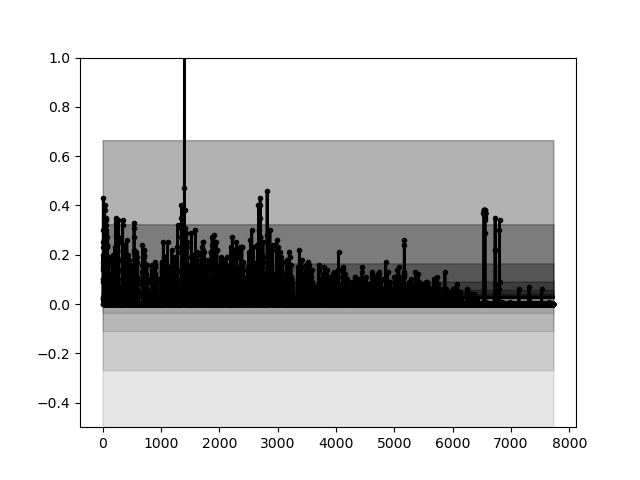
\includegraphics[width=0.45\textwidth]{images/mvskp.png}\end{center}
\end{frame}


\begin{frame}
	\frametitle{Kwartet Anscombe’a}
	Danych jest 11 par punktów $(x, y)$ które mają następujące parametry statystyczne:
	\begin{description}
		\item[średnia x] 9
		\item[wariancja x] 11
		\item[średnia y] 7.5
		\item[wariancja y] 4.125
		\item[korelacja x i y] 0.816
		\item[prosta regresji] 	y = 3 + 0.5x
	\end{description}
\end{frame}
\begin{frame}
	\frametitle{Kwartet Anscombe’a}
	\begin{center}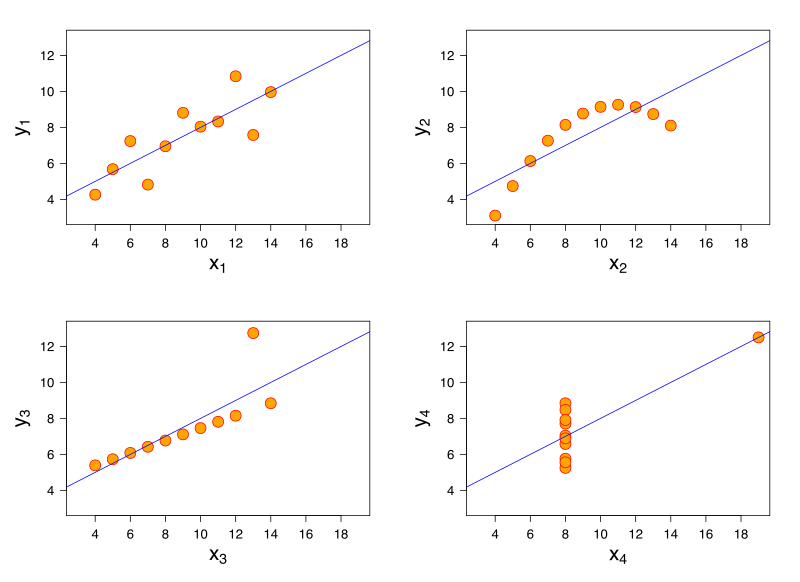
\includegraphics[width=0.6\textwidth]{images/Ansc.png}\end{center}
	{\tiny https://en.wikipedia.org/wiki/File:Anscombe\%27s\_quartet\_3.svg, User:Schutz + User:Avenue, CC SA 3}
\end{frame}
\begin{frame}
	\frametitle{Statystki porządkowe (ang. order statistics)}
	\begin{enumerate}
		\item Mediana
		\item Kwartyle
		\item Percentyle
	\end{enumerate}
\vskip 0.5cm
$\begin{bmatrix}	-2. &   0.5 &  0.71 &  0.6  &  0.7  & -2.1  &  0.59 & 0.51 \end{bmatrix}$
\vskip 0.5cm
$\begin{bmatrix}	-2.1  & -2.  &   0.5  &  0.51  & 0.59  & 0.6 &   0.7   & 0.71 \end{bmatrix}$
\vskip 0.5cm
\begin{description}
	\item[średnia] -0.06125
	\item[mediana] 0.55
\end{description}
\end{frame}
\begin{frame}
	\frametitle{Statystki porządkowe (ang. order statistics) -- wykres pudełkowy (ang. boxplot)}
	\begin{enumerate}
		\item 	$\begin{bmatrix}	-2. &   0.5 &  0.71 &  0.6  &  0.7  & -2.1  &  0.59 & 0.51 \end{bmatrix}$
		\item 100 punktów z rozkładu równomiernego (ang. uniform) $\langle 0, 1\rangle $
		\item 100 punktów ze standardowego rozkładu normalnego (ang. standard normal distribution)
	\end{enumerate}
	\begin{center}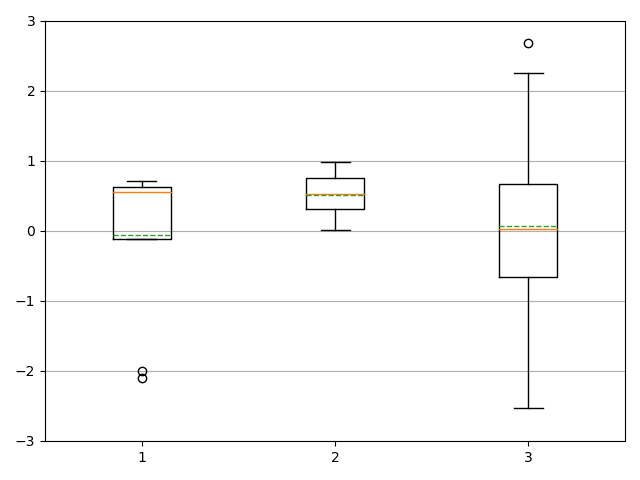
\includegraphics[width=0.4\textwidth]{images/box.png}\end{center}
\end{frame}


\begin{frame}
	\frametitle{Weryfikacja z wykorzystaniem statystyk}
	$\rightarrow$ Algorytm Median Absolute Deviation (MAD)
	\begin{center}
		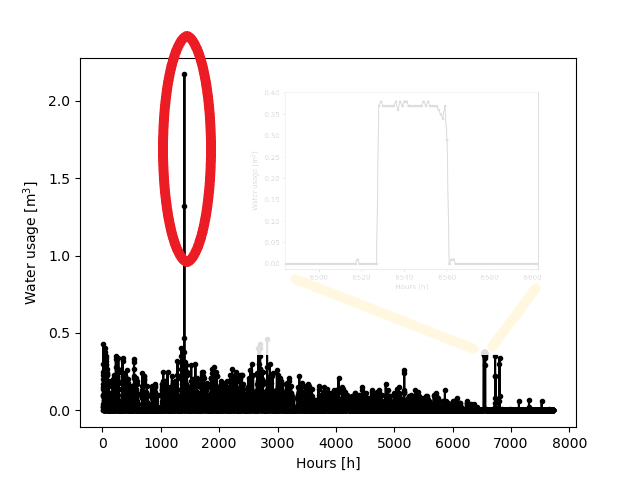
\includegraphics[width=0.5\textwidth]{images/ano1.png}
	\end{center}
\end{frame}
\begin{frame}
	\frametitle{Algorytm Median Absolute Deviation (MAD)}
	\begin{enumerate}
		\item<1-> Dane (przykładowe odczyty) $\mathbf{x} = \begin{bmatrix} 			x_1, x_2, \dots, x_n 		\end{bmatrix}$\\
		{\ttfamily\tiny
		x = [1383.464      1384.9871     1386.6281     1388.142      1389.766
		1391.188      1392.796      1394.144      1395.4139     1396.488
		1398.209      1500.011 1230.793 1549.475 1399.6281
		1238.033 1400.318 1249.4 1400.764      1363.806
		1356.909 1287.488 1402.229      1403.588      1405.167
		1406.427     ]}
		\item<3-> $m = \text{median}(\mathbf{x})$
		\item<4-> $d_i = |x_i - m| \quad \mathbf{d} = \begin{bmatrix} 			d_1, d_2, \dots, d_n 		\end{bmatrix}$
		\item<5-> $T_{\text{MAD}} = \text{median}({\mathbf{d}})$
		\item<6-> $T = 3\times T_{\text{MAD}}$, $d_i > T \rightarrow$ błędny pomiar
	\end{enumerate}
	\only<2>{\begin{center}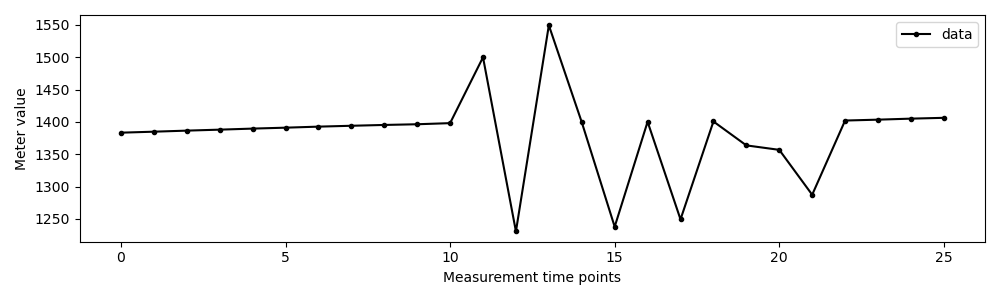
\includegraphics[width=0.65\textwidth]{images/mad1.png}\end{center}}
	\only<3>{\begin{center}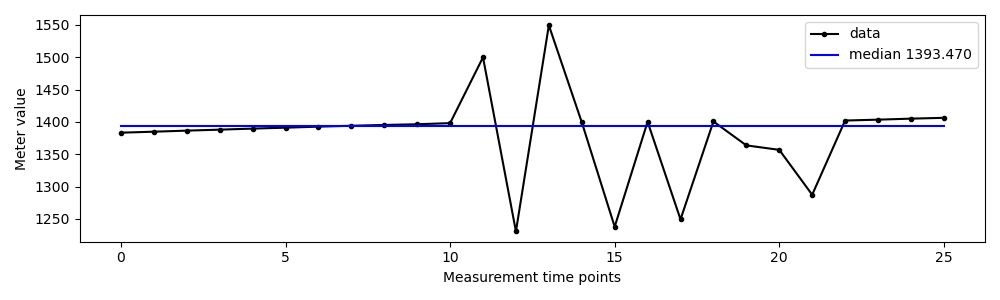
\includegraphics[width=0.65\textwidth]{images/mad2.png}\end{center}}
	\only<4>{\begin{center}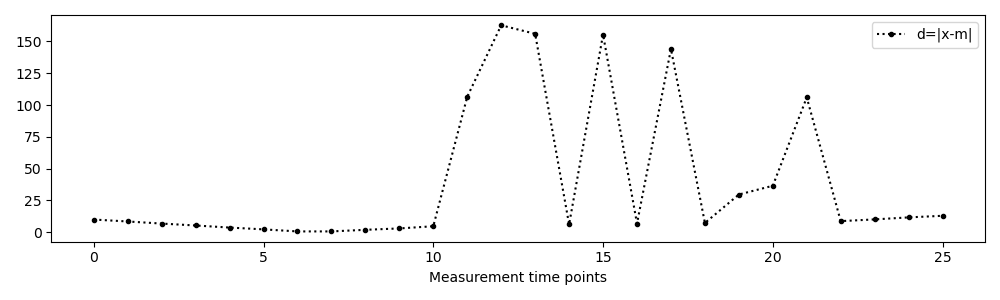
\includegraphics[width=0.65\textwidth]{images/mad3.png}\end{center}}
	\only<5>{\begin{center}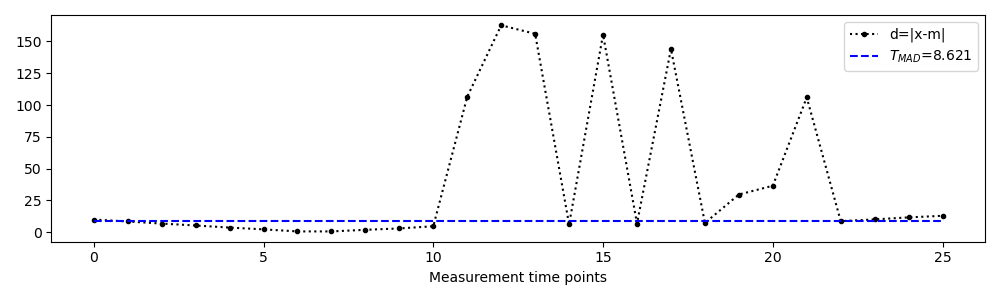
\includegraphics[width=0.65\textwidth]{images/mad4.png}\end{center}}
	\only<6>{\begin{center}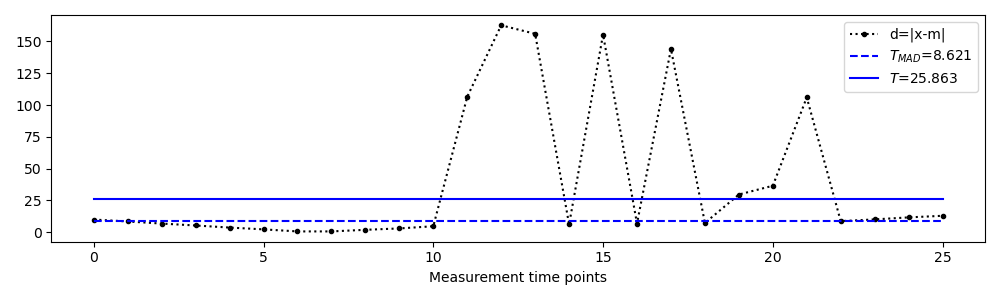
\includegraphics[width=0.65\textwidth]{images/mad5.png}\end{center}}
	\only<7>{\begin{center}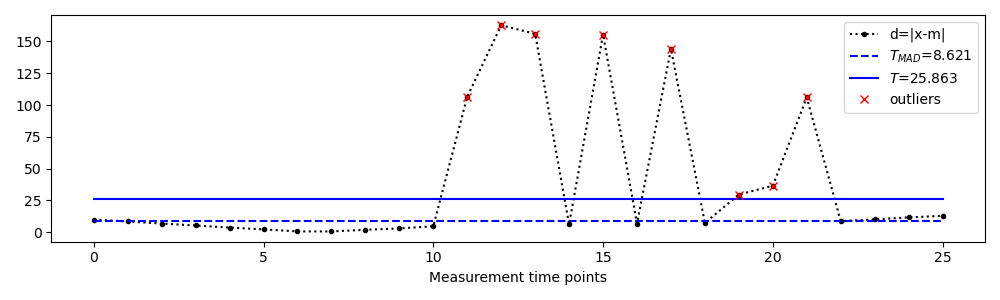
\includegraphics[width=0.65\textwidth]{images/mad6.png}\end{center}}
	\only<8>{\begin{center}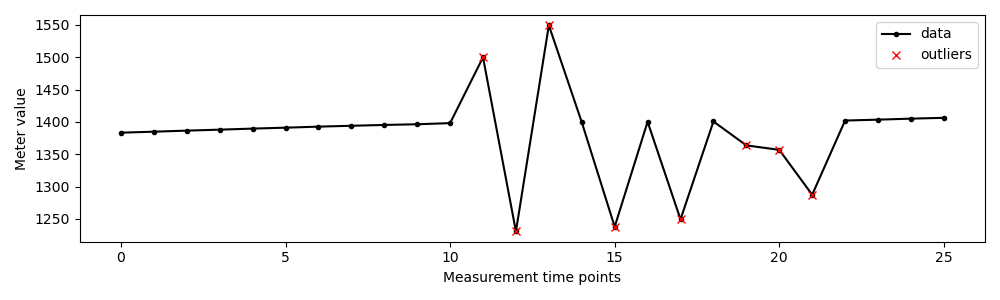
\includegraphics[width=0.65\textwidth]{images/mad7.png}\end{center}}
	\only<9>{\begin{center}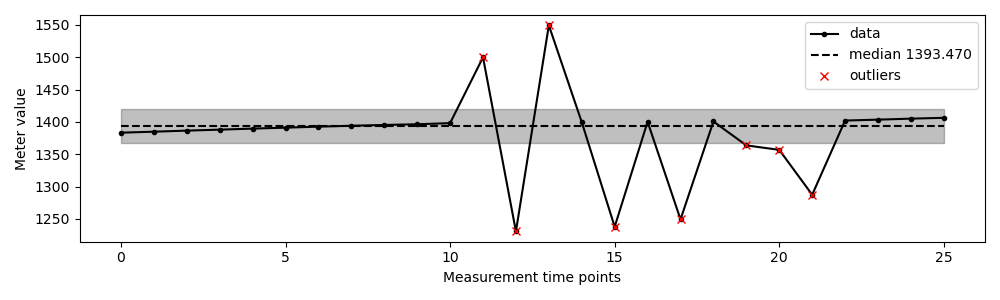
\includegraphics[width=0.65\textwidth]{images/mad8.png}\end{center}}
\end{frame}

\begin{frame}
	\frametitle{Algorytm MAD -- przykłady}
	\begin{center}
		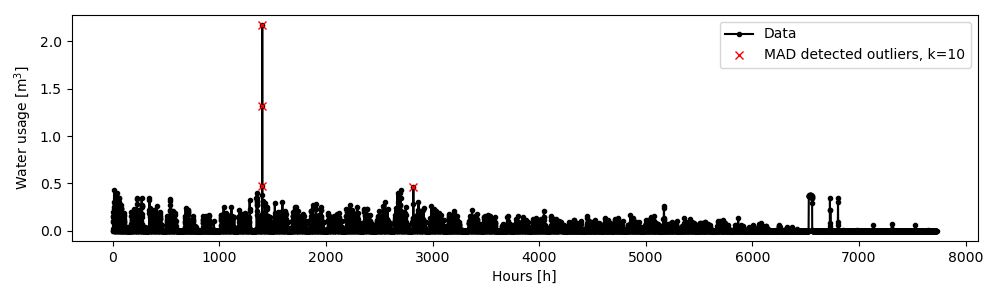
\includegraphics[width=0.65\textwidth]{images/first_cats_mad.png}\\
		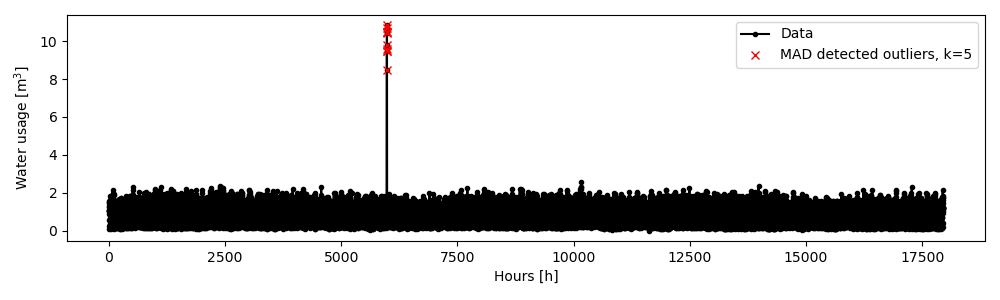
\includegraphics[width=0.65\textwidth]{images/nz_1out_mad.png}
	\end{center}
\end{frame}
\begin{frame}
	\frametitle{Algorytm MAD -- przykłady}
	\begin{center}
		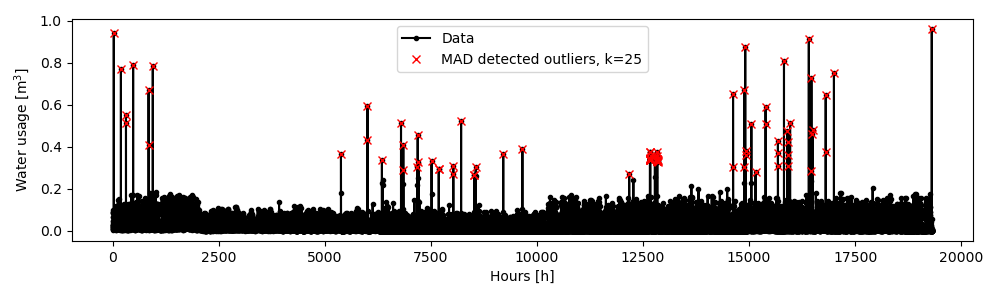
\includegraphics[width=0.65\textwidth]{images/manyout_mad.png}\\
		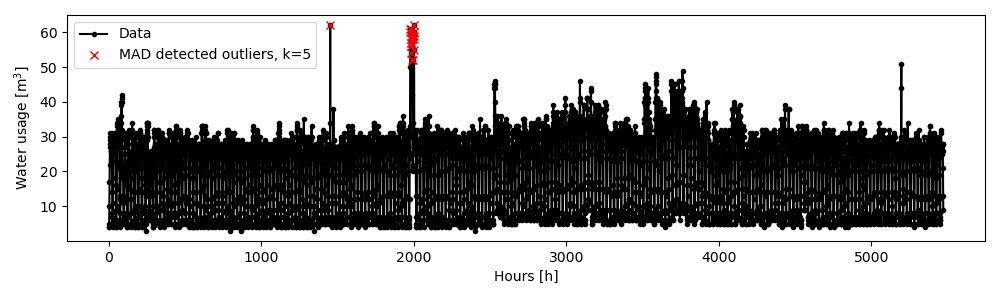
\includegraphics[width=0.65\textwidth]{images/big_pattern2_mad.png}
	\end{center}
\end{frame}

\begin{frame}
	\frametitle{Weryfikacja statystyczna -- outliery}
	\begin{enumerate}
		\item Wykrywanie danych odstających (ang. outliers)
			\begin{enumerate}
				\item ,,odstających'' $\approx$ spoza zakresu danych
				\item MAD (i wiele innych algorytmów)\footnote{\tiny scikit-learn.org/stable/auto\_examples/miscellaneous/plot\_anomaly\_comparison.html, scikit-learn devs, BSD}
			\end{enumerate}
		\item Weryfikacja
			\begin{enumerate}
				\item Wyizolowanie pomiarów błędnych -- błędy urządzeń
				\item Wykrycie anomalii i zmian trendu 
			\end{enumerate}
	\end{enumerate}
	\begin{center}
		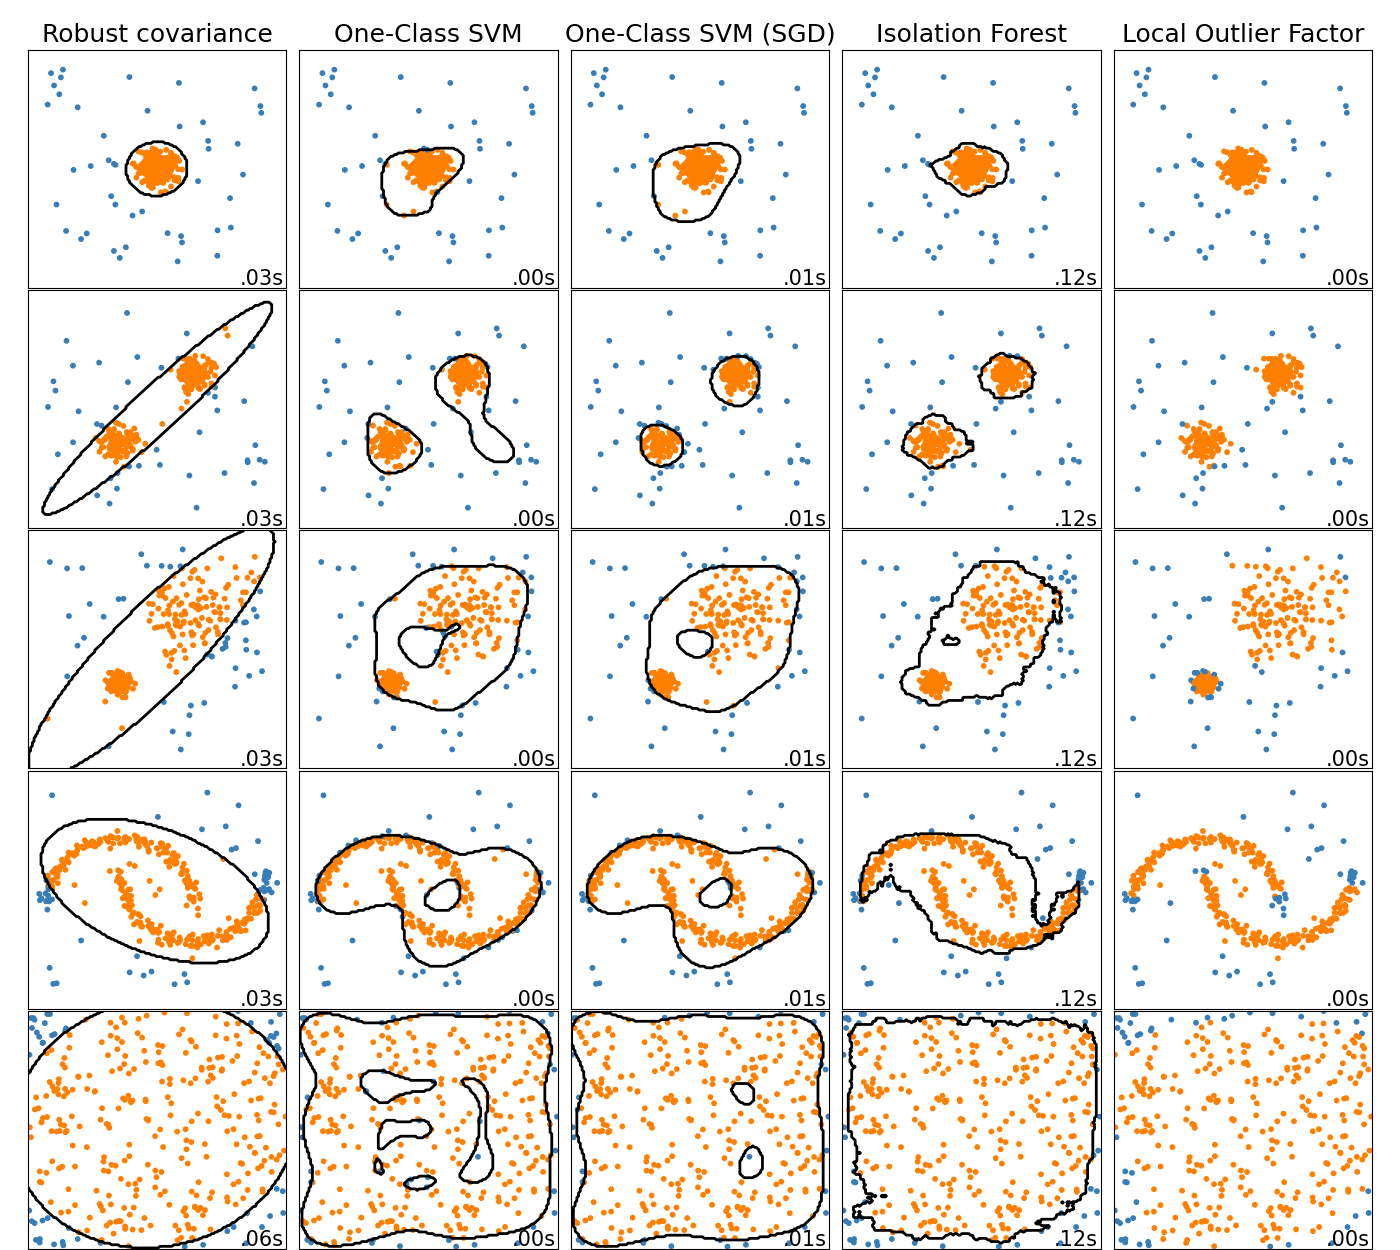
\includegraphics[width=0.27\textwidth]{images/sphx_glr_plot_anomaly_comparison_001.png}
	\end{center}
\end{frame}


\section{Weryfikacja statystyczna -- RX}


\begin{frame}
	\frametitle{Weryfikacja z wykorzystaniem statystyk ,,strikes back''}
	$\rightarrow$ Algorytm Reed-Xiaoli (RX)
	\begin{center}
		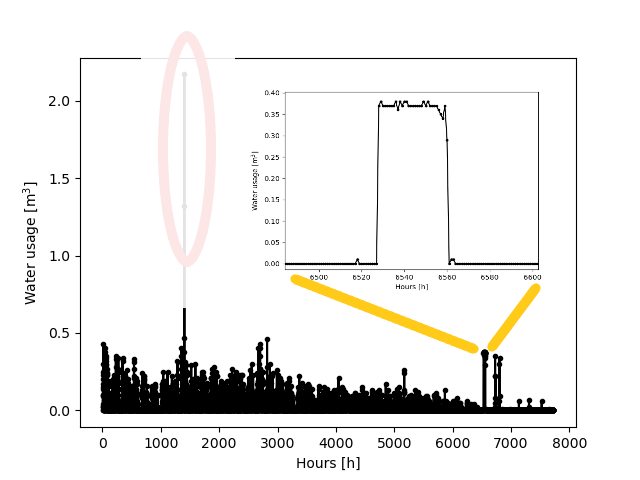
\includegraphics[width=0.5\textwidth]{images/ano2.png}
	\end{center}
\end{frame}

\begin{frame}
	Dlaczego średnia (i inne statystyki np. wariancja) jest dobra?
	\begin{enumerate}
		\item<2-> Łatwa do policzenia
		\item<3-> Znane właściwości 
		\item<4-> Element wnioskowania statystycznego, część bardziej złożonych metod
	\end{enumerate}
	\only<5->{\vskip 0.5 cm
		\begin{description}
			\item[outlier] wartość spoza rozkładu danych, prawdopodobnie błędna - np. błąd urządzenia rejestrującego
			\item[anomalia] wartość z rozkładu danych, ale rzadka -- np. wyciek z instalacji
		\end{description}}
\end{frame}

\begin{frame}
	\frametitle{Wyjście poza pojedyncze punkty danych}
	\begin{center}
		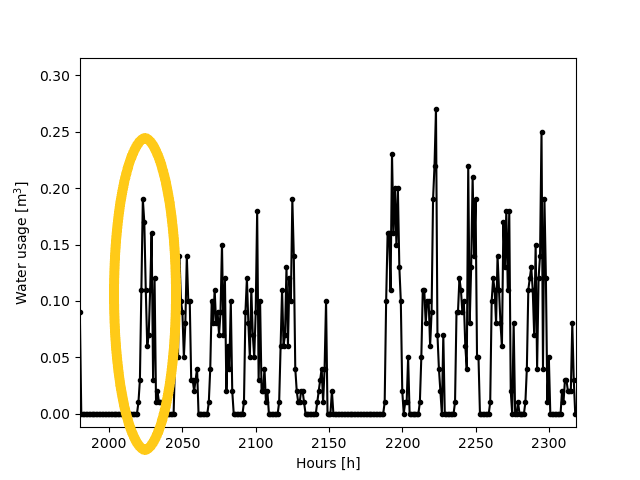
\includegraphics[width=0.6\textwidth]{images/sig1ddd_mark.png}
	\end{center}
\end{frame}

\begin{frame}[fragile]
	\frametitle{Okresy dobowe}
	\begin{enumerate}
		\item Wykorzystujemy właściwości sygnału -- okresowość dobową\\
\begin{verbatim}
	[[4.43 4.77 6.1 ... 7.97 4.85 4.29]
	[4.22 4.18 5.18 ... 9.1  6.37 5.06]
	[4.86 5.9  6.54 ... 8.92 6.54 5.19]
					...
	[2.72 2.52 2.66 ... 9.17 6.59 4.8 ]
	[3.51 2.9  2.52 ... 8.79 5.34 3.59]
	[2.62 2.72 2.57 ... 9.71 6.01 3.41]]
\end{verbatim}
		$X = \begin{bmatrix}
			x_{ij}
		\end{bmatrix} \quad i\: \text{dni}\: j\: \text{godziny,}\quad \mathbf{x}_i\: \text{i-ta doba}$
		\item<2-> Anomalia $\rightarrow$ ,,nietypowe zachowanie''
		\item<3-> ,,Zachowanie'' $\rightarrow$ średnia dobowa $\bar{\mathbf{x}} = \begin{bmatrix}
			\bar{x}_j 
		\end{bmatrix}\quad \bar{x}_j = \frac{1}{n}\sum_{i=1}^n x_{ij}$
		\item<4-> ,,Nietypowe'' $\rightarrow$ duża odległość od średniej $\| \bar{\mathbf{x}} - \mathbf{x}_i \| = \sqrt{\sum_{j=1}^{24}(\bar{x}_j - x_{ij})^2}$ 
	\end{enumerate}
\end{frame}
\begin{frame}
	\frametitle{Problem?}
	\begin{center}
		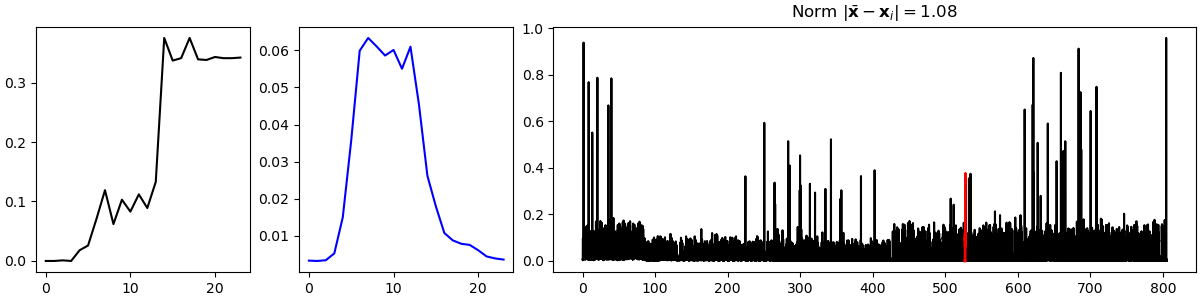
\includegraphics[width=0.75\textwidth]{images/manyout_X_527.png}\\
		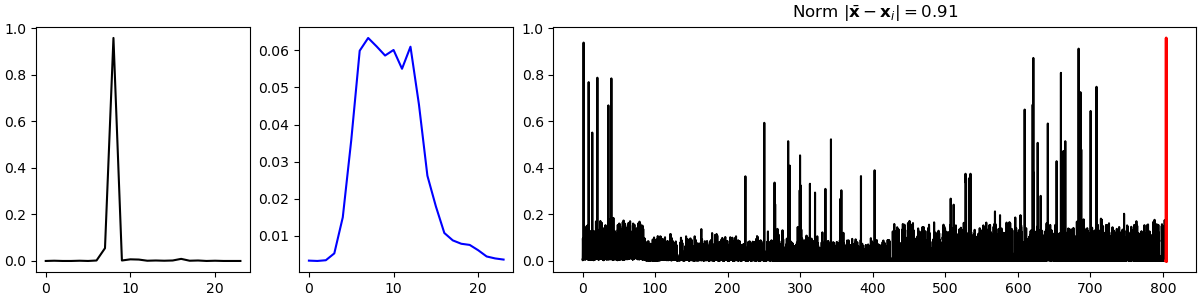
\includegraphics[width=0.75\textwidth]{images/manyout_X_804.png}
	\end{center}
\end{frame}
\begin{frame}
	\frametitle{Problem?}
	\begin{center}
		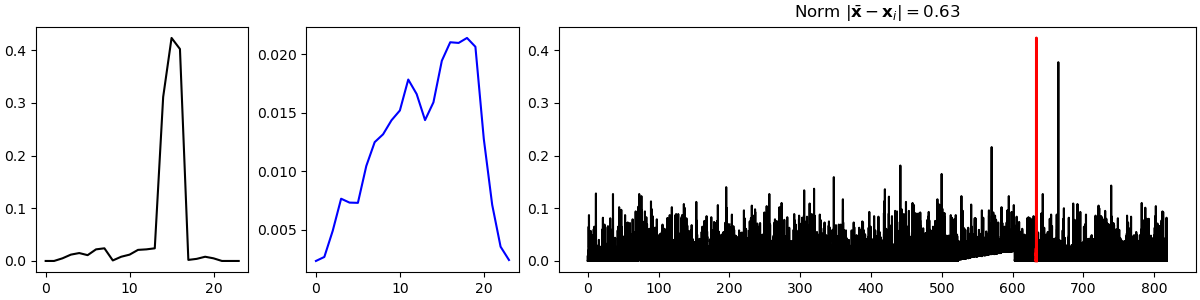
\includegraphics[width=0.75\textwidth]{images/leakano_X_633.png}\\
		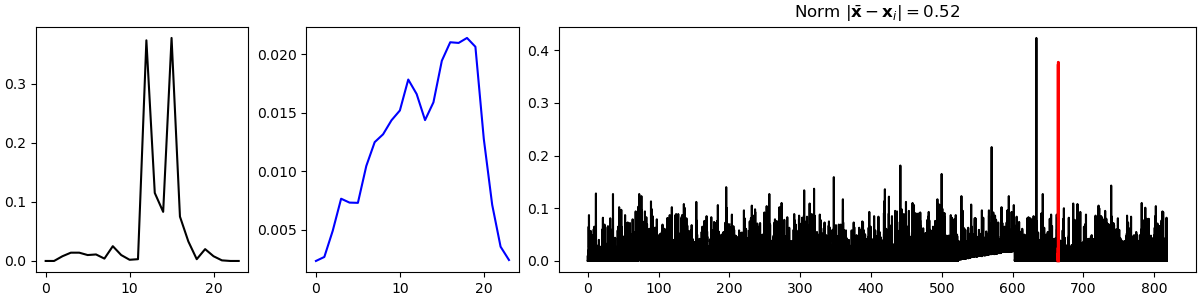
\includegraphics[width=0.75\textwidth]{images/leakano_X_664.png}
	\end{center}
\end{frame}
\begin{frame}
	\frametitle{Odległość od średniej a rozkład danych}
	\begin{center}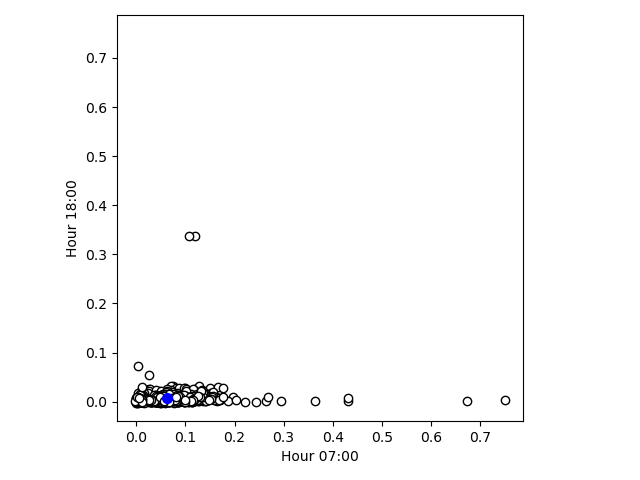
\includegraphics[width=0.6\textwidth]{images/nil.png}	\end{center}
\end{frame}
\begin{frame}
	\frametitle{Odległość od średniej a rozkład danych}
	\begin{center}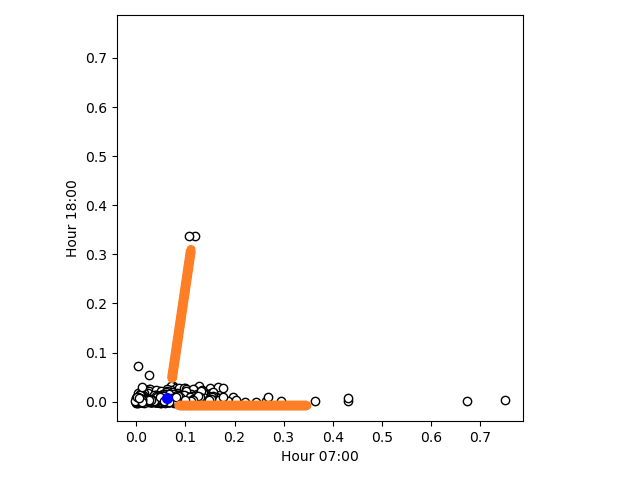
\includegraphics[width=0.6\textwidth]{images/nil1.png}	\end{center}
\end{frame}
\begin{frame}
	\frametitle{Odległość od średniej a rozkład danych}
	\begin{center}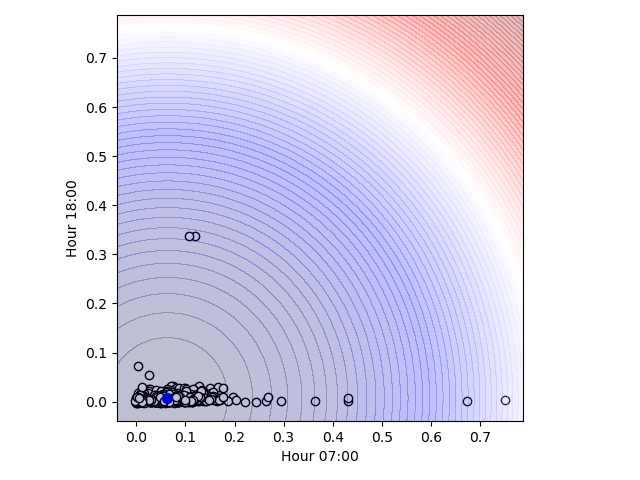
\includegraphics[width=0.6\textwidth]{images/eye.png}	\end{center}
\end{frame}
\begin{frame}
	\frametitle{Odległość od średniej a rozkład danych}
	\begin{center}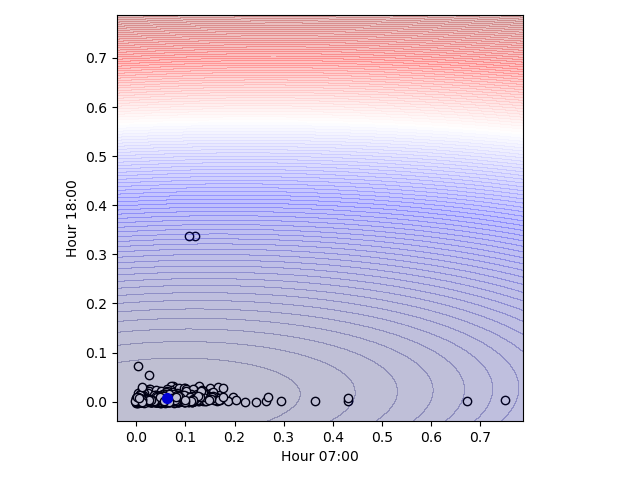
\includegraphics[width=0.6\textwidth]{images/C.png}	\end{center}
\end{frame}
\begin{frame}
	\frametitle{Opis rozkładu -- macierz kowariancji}
	\begin{center}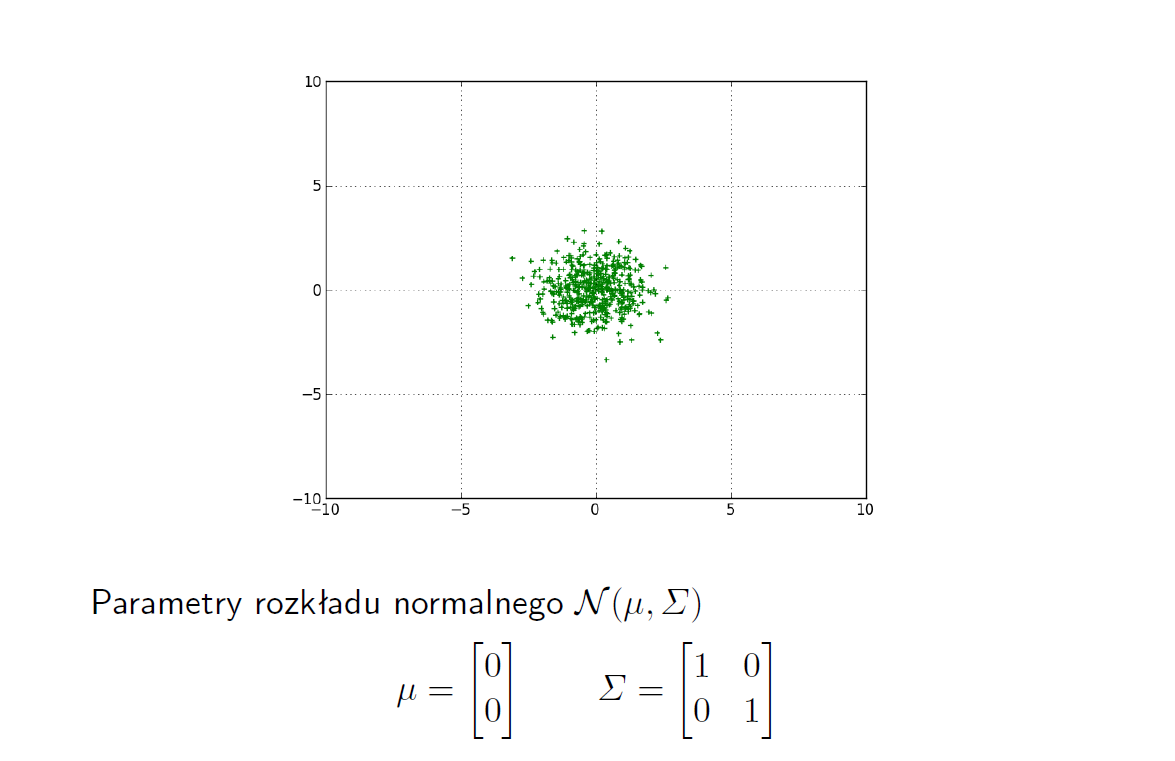
\includegraphics[width=0.6\textwidth]{images/nnomean.png}	\end{center}
\end{frame}
\begin{frame}
	\frametitle{Opis rozkładu -- macierz kowariancji}
	\begin{center}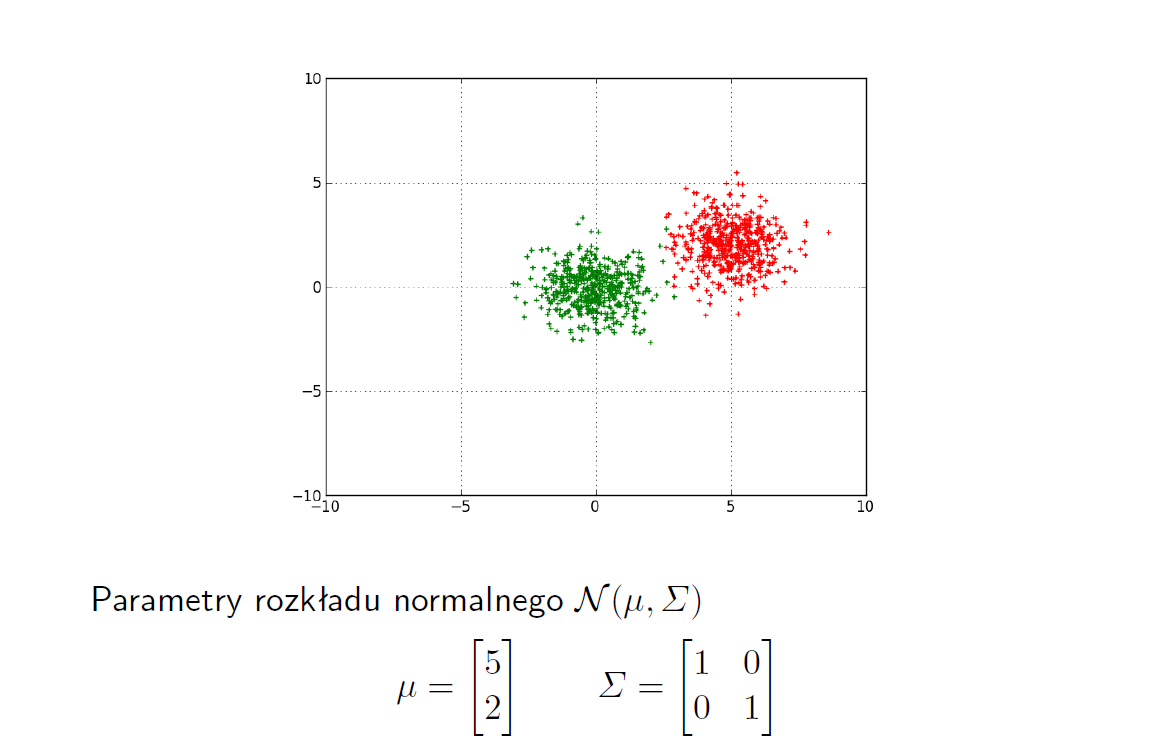
\includegraphics[width=0.6\textwidth]{images/nmean.png}	\end{center}
\end{frame}
\begin{frame}
	\frametitle{Opis rozkładu -- macierz kowariancji}
	\begin{center}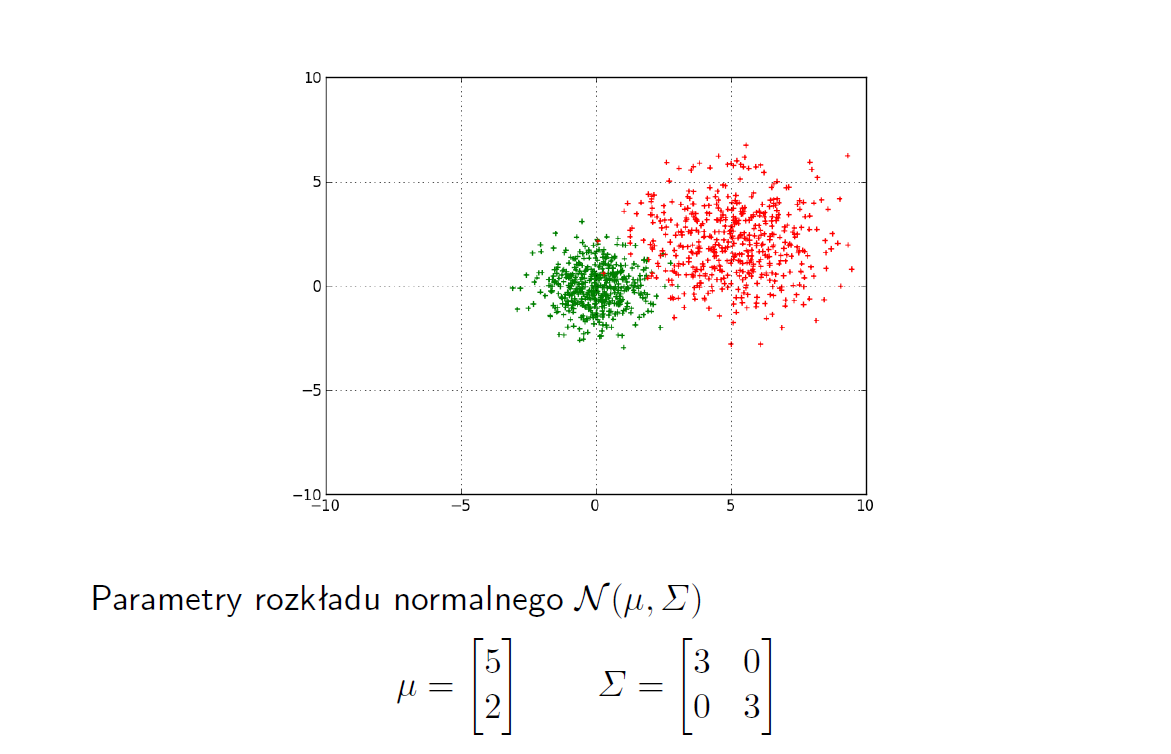
\includegraphics[width=0.6\textwidth]{images/nsphe.png}	\end{center}
\end{frame}
\begin{frame}
	\frametitle{Opis rozkładu -- macierz kowariancji}
	\begin{center}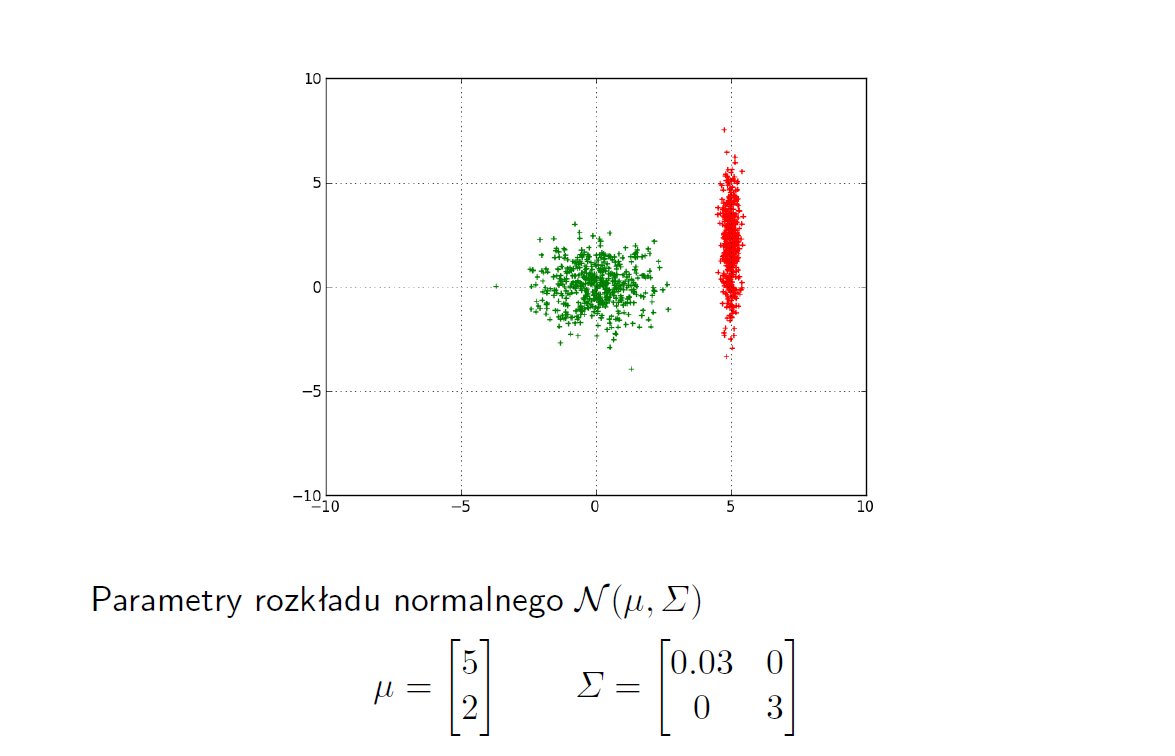
\includegraphics[width=0.6\textwidth]{images/nvar.png}	\end{center}
\end{frame}
\begin{frame}
	\frametitle{Opis rozkładu -- macierz kowariancji}
	\begin{center}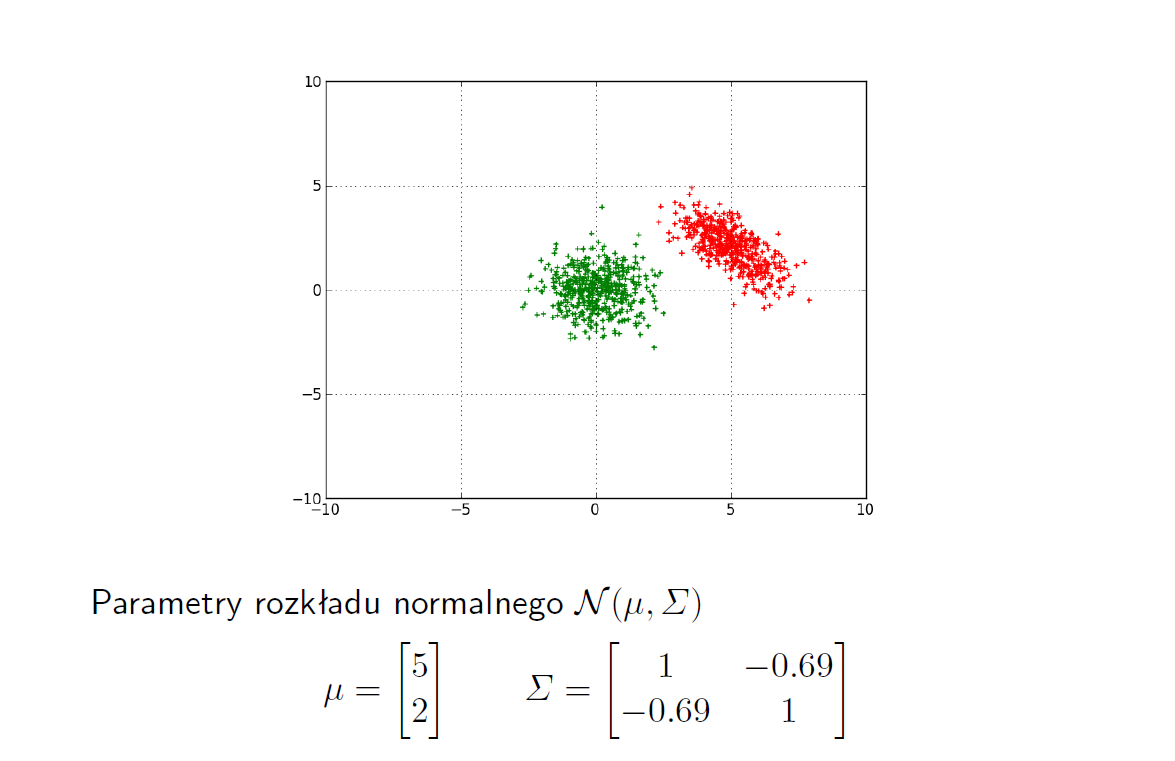
\includegraphics[width=0.6\textwidth]{images/ncov.png}	\end{center}
\end{frame}


\begin{frame}
	\frametitle{Odległość Mahalanobisa}
%	\begin{enumerate}
%		\item<1-> $d_E(\bar{\mathbf{x}}, \mathbf{x}_i) = \| \bar{\mathbf{x}} - \mathbf{x}_i \| = \sqrt{\sum_{j=1}^{24}(\bar{x}_j - x_{ij})^2}=$
%		\item<2-> $= \sqrt{\mathbf{x}\mathbf{x}_i^\top} $
%	\end{enumerate}
	
	\only<1->{$d_E(\bar{\mathbf{x}}, \mathbf{x}_i) = \| \bar{\mathbf{x}} - \mathbf{x}_i \| = \sqrt{\sum_{j=1}^{24}(\bar{x}_j - x_{ij})^2}=$} \only<2->{$ \sqrt{(\bar{\mathbf{x}} - \mathbf{x}_i)(\bar{\mathbf{x}} - \mathbf{x}_i)^\top} = $}
	\only<3->{$ \sqrt{(\bar{\mathbf{x}} - \mathbf{x}_i)I(\bar{\mathbf{x}} - \mathbf{x}_i)^\top}$}
	\vskip 0.2cm
	\only<3->{$I$ -- macierz identyczności }
	\vskip 0.4cm
	\only<4->{$C=\frac{1}{n-1}\sum_{i=1}^n (\mathbf{x}_i - \bar{\mathbf{x}})^\top (\mathbf{x}_i - \bar{\mathbf{x}})$ -- macierz kowariancji danych (ang. sample covariance)}
	\vskip 0.2cm
	\only<5->{$C^{-1}$ -- odwrotność macierzy kowariancji}
	\vskip 0.2cm
	\only<6->{$d_M(\bar{\mathbf{x}}, \mathbf{x}_i)= \sqrt{(\bar{\mathbf{x}} - \mathbf{x}_i)C^{-1}(\bar{\mathbf{x}} - \mathbf{x}_i)^\top} $}
\end{frame}
\begin{frame}
	\frametitle{Odległość Mahalanobisa}
	\begin{center}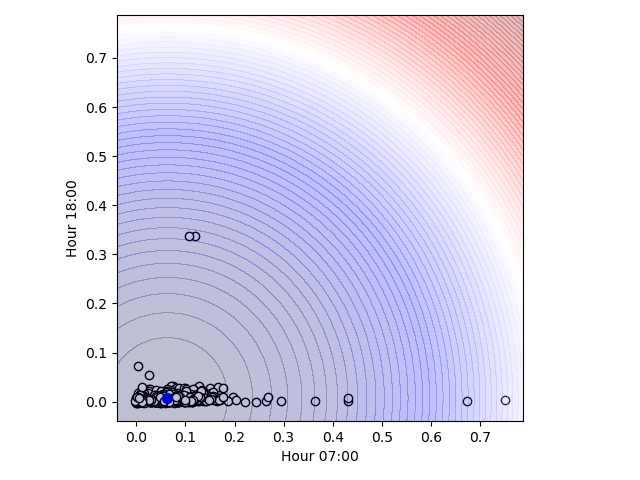
\includegraphics[width=0.48\textwidth]{images/eye.png}	
		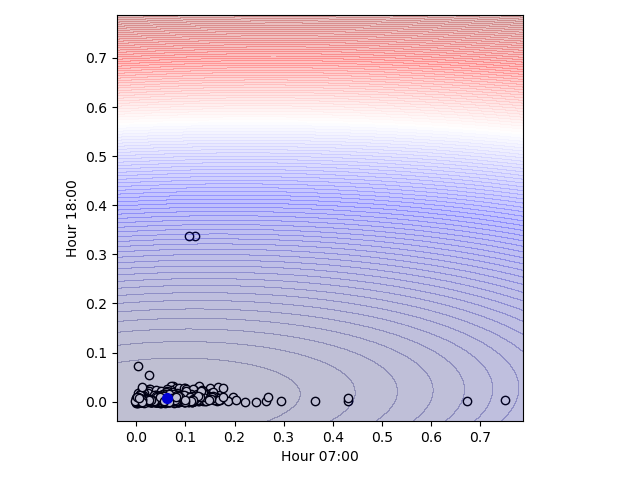
\includegraphics[width=0.48\textwidth]{images/C.png}	\end{center}
\end{frame}



\begin{frame}[fragile]
	\frametitle{Wykrywanie anomalii -- odległość Mahalanobisa}
	\begin{enumerate}
		\item Wykorzystujemy właściwości sygnału -- okresowość dobową\\
		\begin{verbatim}
			[[4.43 4.77 6.1 ... 7.97 4.85 4.29]
			[4.22 4.18 5.18 ... 9.1  6.37 5.06]
			[4.86 5.9  6.54 ... 8.92 6.54 5.19]
			...
			[2.72 2.52 2.66 ... 9.17 6.59 4.8 ]
			[3.51 2.9  2.52 ... 8.79 5.34 3.59]
			[2.62 2.72 2.57 ... 9.71 6.01 3.41]]
		\end{verbatim}
		$X = \begin{bmatrix}
			x_{ij}
		\end{bmatrix} \quad i\: \text{dni}\: j\: \text{godziny,}\quad \mathbf{x}_i\: \text{i-ta doba}$
		\item Anomalia $\rightarrow$ ,,nietypowe zachowanie''
		\item ,,Zachowanie'' $\rightarrow$ średnia dobowa $\bar{\mathbf{x}} = \begin{bmatrix}
			\bar{x}_j 
		\end{bmatrix}\quad \bar{x}_j = \frac{1}{n}\sum_{i=1}^n x_{ij}$ {\color{red} i macierz kowariancji}
		\item ,,Nietypowe'' $\rightarrow$ duża odległość od średniej {\color{red} liczona odległością Mahalanobisa $d_M(\bar{\mathbf{x}}, \mathbf{x}_i)$}
	\end{enumerate}
\end{frame}

\begin{frame}
	\frametitle{Wykrywanie anomalii -- odległość Mahalanobisa $\rightarrow$ algorytm RX}
	\begin{enumerate}
		\item<1-> Mamy dane $X$ $\rightarrow$ średnia $\bar{\mathbf{x}}$, macierz kowariancji $C$
		\item<2-> $\mathbf{x}_i$ jest anomalią jeżeli $d_M(\bar{\mathbf{x}}, \mathbf{x}_i) > T$ \only<3->{\dots ale jak wyliczyć $T$?}\\ \only<4->{\dots dla różnych wartości średniej i m. kowariancji różne $T$ :( }
		\item<5-> Chcielibyśmy wyrazić próg w postaci prawdopodobieństwa, np. anomalia jest jeżeli $\mathbf{x}_i$ ma prawdopodobieństwo np. $\alpha=1\%$, albo 0.1\% \only<6->{\dots a dla $\alpha$ wyznaczyć $T$ automatycznie}
		\item<7-> Wiemy, że jeżeli punkty w $X$ mają rozkład normalny, to  $d_M(\bar{\mathbf{x}}, \mathbf{x}_i)$ ma rozkład $\chi^2$ z $d$-stopniami swobody (w naszym wypadku $d=24$)
		\item<8-> Znając rozkład -- w tym wypadku $\chi^2$ -- możemy wyznaczyć $T$, dla którego prawdopodobieństwo przekroczenia wartości jest $\alpha$, $P(d_M(\bar{\mathbf{x}}, \mathbf{x}_i) > T) = \alpha$
	\end{enumerate}
\end{frame}

\section{Algorytm RX -- przykłady}

\begin{frame}
	Dane sztucznie wygenerowane, rozkład normalny, $d=1$
	\begin{center}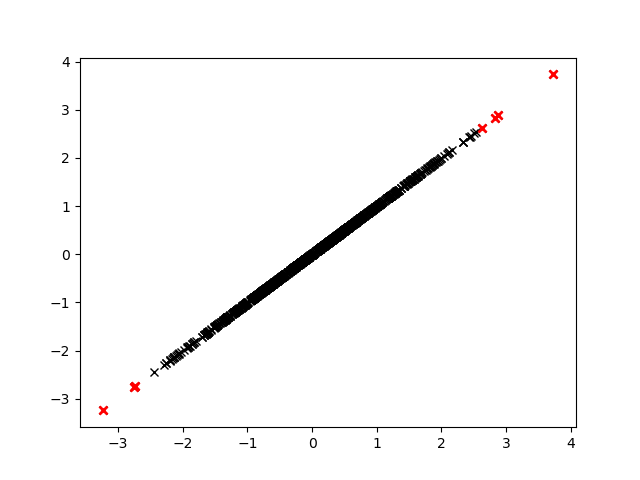
\includegraphics[width=0.49\textwidth]{images/rx1.png}	
		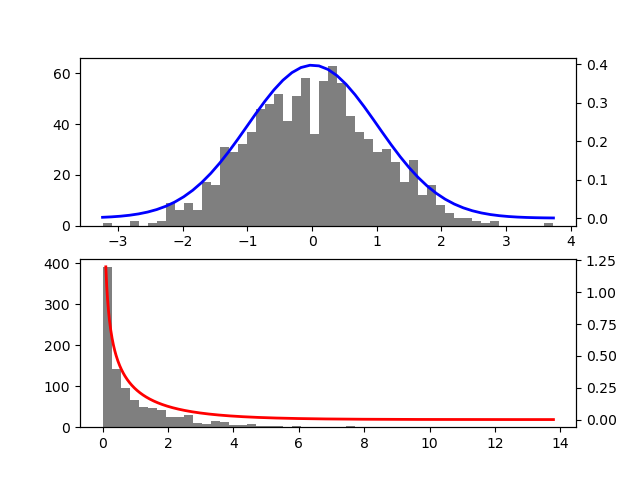
\includegraphics[width=0.49\textwidth]{images/rx1d.png}	\end{center}
\end{frame}
\begin{frame}
	Dane sztucznie wygenerowane, rozkład normalny, $d=2$
	\begin{center}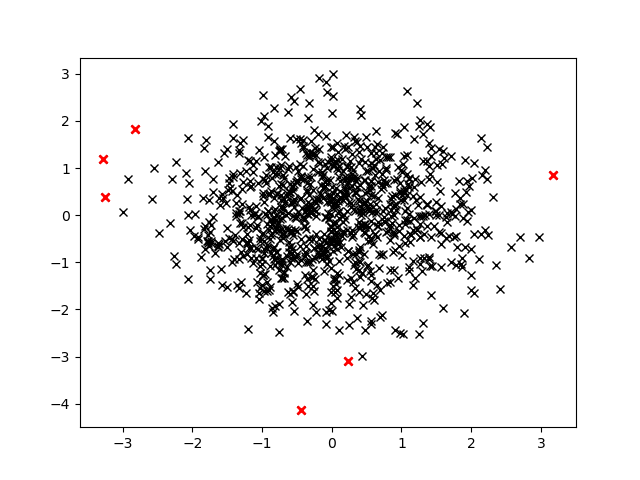
\includegraphics[width=0.49\textwidth]{images/rx2.png}	
		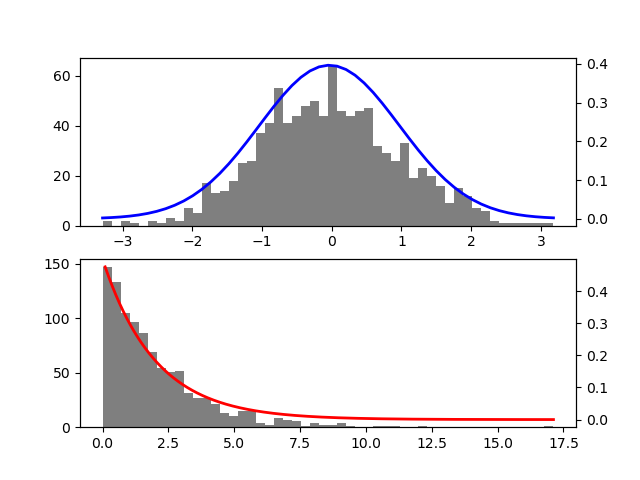
\includegraphics[width=0.49\textwidth]{images/rx2d.png}	\end{center}
\end{frame}
\begin{frame}
	Dane sztucznie wygenerowane, rozkład normalny, $d=50$
	\begin{center}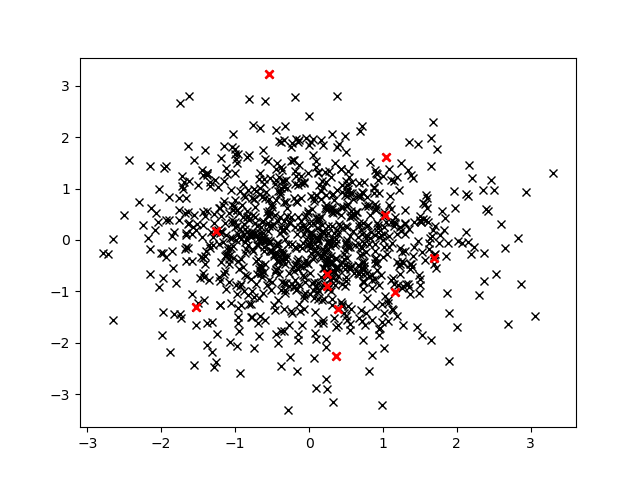
\includegraphics[width=0.49\textwidth]{images/rx50.png}	
		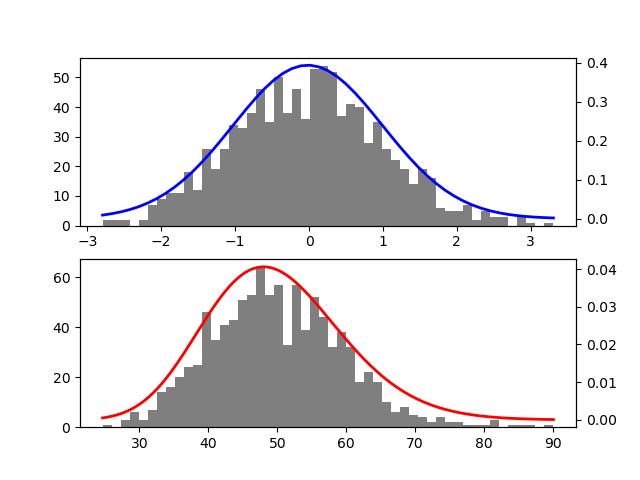
\includegraphics[width=0.49\textwidth]{images/rx50d.png}	\end{center}
\end{frame}
\begin{frame}
	Dane rzeczywiste (monitoring przemysłowy), rozkład -- ?, $d=1$
	\begin{center}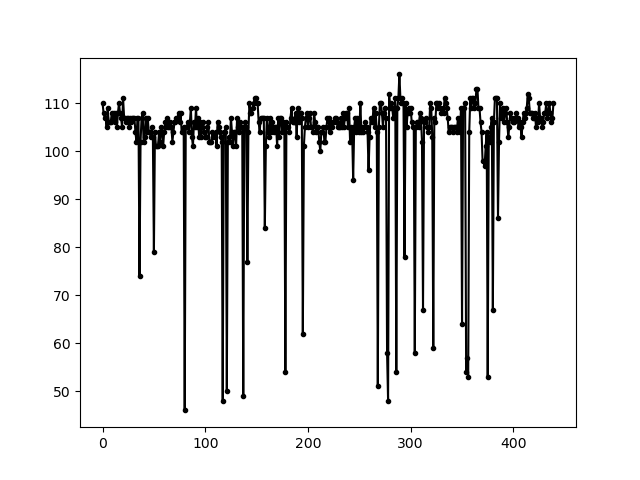
\includegraphics[width=0.49\textwidth]{images/rxh.png}	
		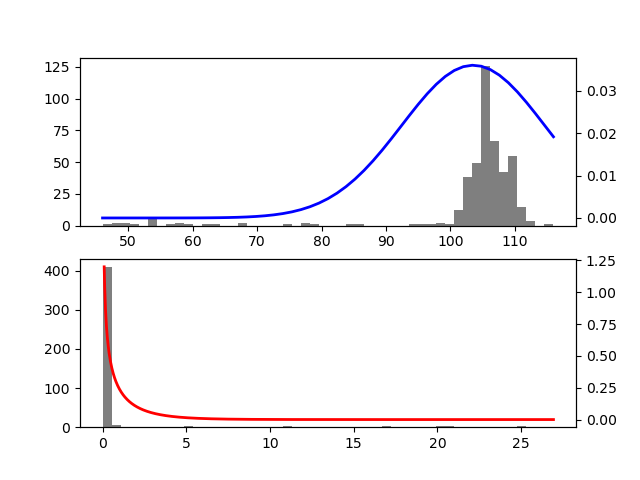
\includegraphics[width=0.49\textwidth]{images/rxhd.png}	\end{center}
\end{frame}
\begin{frame}
	Dane rzeczywiste (monitoring przemysłowy), rozkład -- ?, $d=1$
	\begin{center}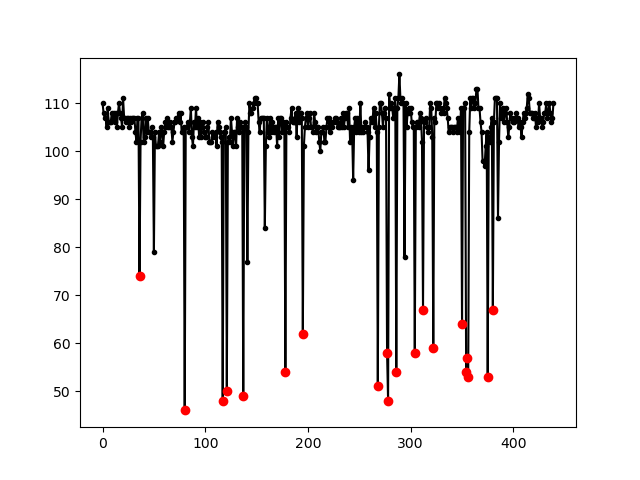
\includegraphics[width=0.49\textwidth]{images/rxha.png}	
		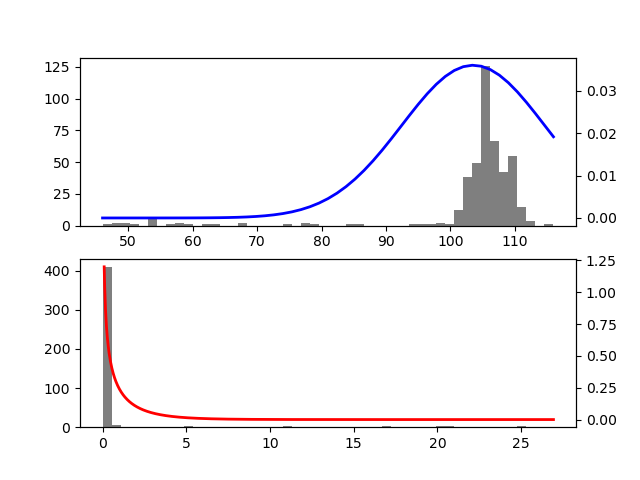
\includegraphics[width=0.49\textwidth]{images/rxhd.png}	\end{center}
\end{frame}
\begin{frame}
	Dane rzeczywiste (zdjęcie hiperspektralne), rozkład -- ?, $d=100$
	\begin{center}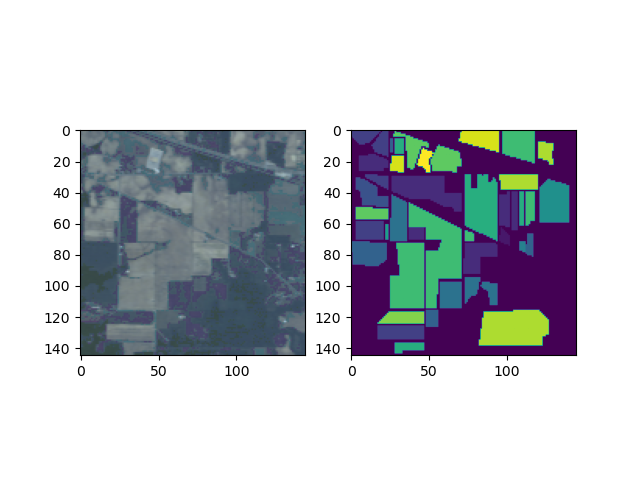
\includegraphics[width=0.69\textwidth]{images/rxhsi.png}	\end{center}
\end{frame}
\begin{frame}
	Dane rzeczywiste (zdjęcie hiperspektralne), rozkład -- ?, $d=100$
	\begin{center}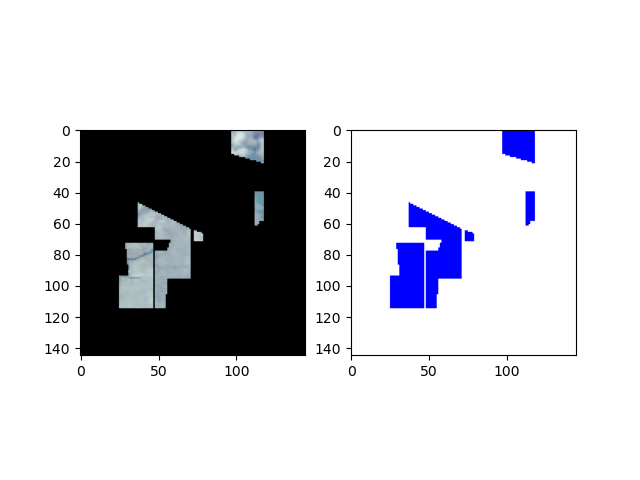
\includegraphics[width=0.49\textwidth]{images/rxhsi1.png}	
		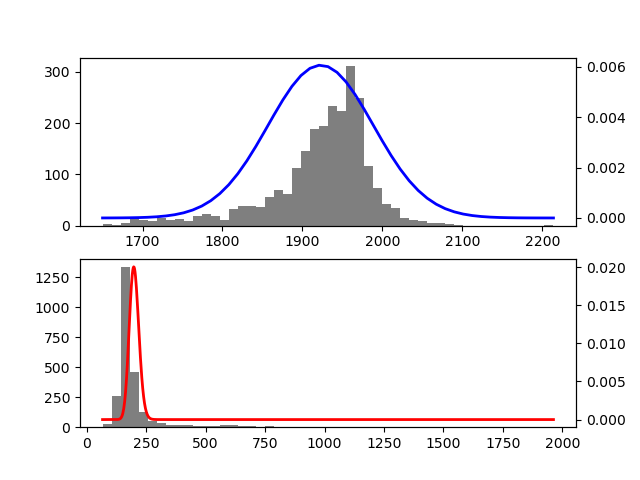
\includegraphics[width=0.49\textwidth]{images/rxhsi1d.png}	\end{center}
\end{frame}
\begin{frame}
	Dane rzeczywiste (zdjęcie hiperspektralne), rozkład -- ?, $d=100$
	\begin{center}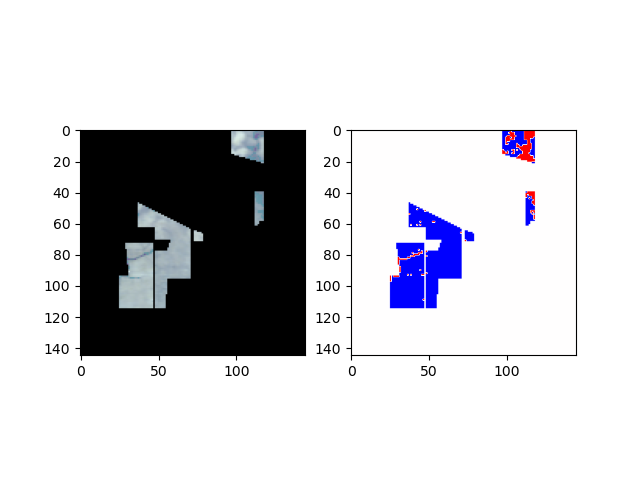
\includegraphics[width=0.49\textwidth]{images/rxhsi1a.png}	
		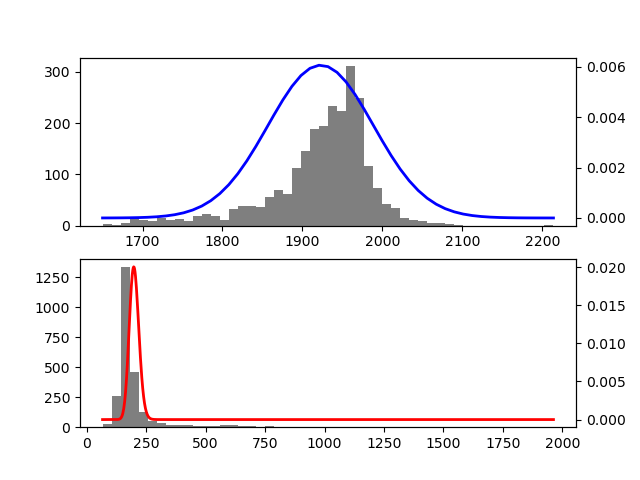
\includegraphics[width=0.49\textwidth]{images/rxhsi1d.png}	\end{center}
\end{frame}

\begin{frame}
	\frametitle{Wykrywanie anomalii, algorytm RX, podsumowanie}
	\begin{enumerate}
		\item<1-> Anomalie a outliery
		\item<2-> Elementy (RX):
			\begin{enumerate}
				\item Model -- rozkład normalny, opisany średnią i macierzą kowariancji (parametry)
				\item Algorytm -- odległość Mahalanobisa, wykorzystanie znanego rozkładu $\chi^2$ (parametry wejściowe, wyjście)
				\item Teoria -- prawdopodobieństwo i statystyka
			\end{enumerate}
		\item<3-> Rozwinięcia
			\begin{enumerate}
				\item Mixture of Gaussians (MoG)
				\item Principal Component Analysis (PCA) 
				\item Hidden Markov Models (HMM)
			\end{enumerate}
		\item<4-> Alternatywy -- np. sieci neuronowe
	\end{enumerate}
\end{frame}


% several examples - from file 

% chisquare distributions varia, finallement just give alpha 
% which two select, but why two? can take all 
% formulation with covariance matrix and detection
% see detection on example data 


%\section{Weryfikacja statystyczna -- rozwinięcia}


% turns out covariance matrix is good for zmienność - jaka jest największa zmienność obecna w danych, bez szukanai par - 1d plot with see
% można dodać drugi kierunek, 2d plot with see 
% generalissimus anomaly detection summary and outlooke 
% come case study of different, moar complex - include the intro of MoG 
% summario of the great body of knowledge laid in front of ye
% generalization - image ze strzałkami - statistical tests, clustering, more advanced models, more adbanced projections and visualizations



% database key - retention, backups, transactions
% sql 
% working example
% sql i inne 


% min. data sources -- 
% min. data bases 
% transakcje itp 



%\begin{frame}
%	\frametitle{Analiza danych -- 101}
%	\begin{enumerate}
%	\item Inspekcja założeń
%		\begin{itemize}
%		\item Usuwanie danych odstających (\emph{outliers}) np. MAD
%		\item Dopasowanie znanego modelu np. LSQ, RANSAC
%		\end{itemize}
%	\item Analiza i wizualizacja -- prosta
%		\begin{itemize}
%		\item Średnia, mediana, \dots, macierz kowariancji
%		\item \emph{plot, scatterplot, histogram, boxplot}
%		\end{itemize}	
%	\item Analiza i wizualizacja -- złożona
%		\begin{itemize}
%		\item Wykrywanie anomalii (RX)
%		\item Grupowanie (\emph{clustering}; MoG, KMeans, hierarchiczne)
%		\item PCA (\emph{Principal Component Analysis}, analiza składowych głównych)
%		\end{itemize}
%	\item Budowa modeli
%		\begin{itemize}
%		\item Klasyfikacji, detekcji, predykcji, wnioskowania $\rightarrow$ wykład 3, 4, 5
%		\end{itemize}
%	\end{enumerate}
%\end{frame}
%
%
%\begin{frame}
%	\frametitle{Analiza danych -- 101 -- podsumowanie}
%	\begin{enumerate}
%	\item Wizualizacje \emph{plot, histogram, scatterplot}
%	\item Statystyki opisowe: średnia, odchylenie standardowe (+\emph{coefficient of variation, CV}), skośność, kurtoza
%	\item Opis szeregu uporządkowanego: mediana, kwantyle (kwartyle, percentyle), Q1, Q3, IQR
%	\item Wizualizacja \emph{boxplot}
%	\item Rozkład normalny
%	\item Korelacja, macierz kowariancji
%	\item \emph{RX anomaly detector}
%	\item model mieszaniny rozkładów \emph{Mixture of Gaussians} MoG, EM
%	\item PCA
%	\item KMeans
%	\end{enumerate}
%\end{frame}
%
%
%\begin{frame}
%	\frametitle{Analiza danych -- poziom zaawansowany}	
%	\begin{enumerate}
%	\item Inne rodzaje danych (szeregi czasowe, tekst, grafy, \dots)
%	\item Zaawansowana analiza statystyczna -- rozkłady, testy statystyczne
%	\item ,,Artystyczna'' wizualizacja
%	\item Zaawansowane algorytmy analizy
%		\begin{itemize}
%		\item Grupowanie inne niż KMeans (np. hierarchiczne, t-SNE)
%		\item Rzutowanie inne niż PCA (np. Fourier, falki, ICA)
%		\item Różne metody wykrywania/usuwania anomalii, normalizacji itp
%		\item Rozbudowane modele wnioskowania i decyzji
%		\end{itemize}
%	\end{enumerate}
%\end{frame}


\end{document}

